% !TeX program = lualatex
\documentclass[10pt, a4paper]{article}

\usepackage{GeneralHeaders}
\usepackage{GregorioHeaders}
\usepackage{ColumnHeaders}

\usepackage[left=1cm, right=1cm, top=1cm, bottom=2cm]{geometry}

\begin{document}

\title{Ad Completorium}
\author{}
\date{}

% \begin{center}

  \thispagestyle{empty}

  \phantom{Ad maiorem Dei gloriam}

  \vspace{7cm}

  {\Huge\scshape \MakeUppercase{Ad Completorium}}

  \vspace{1cm}

  {\huge \textit{Compline}}

  \vfill

  {\Large \GreColored{Sydneyen}

  \vspace{0.5cm}

  {\scshape\GreColored{mmxxv}}}

\end{center}

\newpage
  \thispagestyle{empty}
  \phantom{Ad maiorem Dei gloriam}
\newpage

%
% \begin{center}
  \phantom{Ad maiorem Dei gloriam}

  \vspace{1.25cm}

  {\Huge\scshape\textls[150]{\MakeLowercase{Ordinarium}}}

  \vspace{0.50cm}

  {\Large\itshape The Ordinary}

  \vspace{1.25cm}
\end{center}

\bisubsection{Ad ritum initialem}{Introductory rite}\pdfbookmark[section]{Ad ritum initialem}{ad-ritum-initialem}

\bimusichangingdoubleversicle[Tonus communis:][Common tone:]{\gregorioscore{../ToniCommunes/4121-or--deus_in_adiutorium_(tonus_ferialis)--solesmes_2000s.gabc}}{\VbarT O God, \GreColored{\grecross}\, come to our aid.

\RbarT O Lord, make haste to help us.

Glory be to the Father and to the Son and to the Holy Spirit. As it was in the beginning, is now, and ever shall be, world without end. Amen. Alleluia. \GreColored{Alleluia \textit{is omitted during Lent.}}}

\bimusichangingdoubleversicle[Tonus sollemnis:][Solemn tone:]{\gregorioscore{../ToniCommunes/7864-or--deus_in_adiutorium_(ad_lm_et_vesp._in_sollemnitatibus)--solesmes_2000s.gabc}}{\VbarT O God, \GreColored{\grecross}\, come to our aid.

\RbarT O Lord, make haste to help us.

Glory be to the Father and to the Son and to the Holy Spirit. As it was in the beginning, is now, and ever shall be, world without end. Amen. Alleluia. \GreColored{Alleluia \textit{is omitted during Lent.}}}

\verticalspacer

\biinstruction{Postea laudabiliter fit conscientiæ discussio, quæ in celebratione commune inseri potest in actum pænitentialem, iuxta forumulas in Missa adhibitas. \textcolor{black}{Confiteor} infra indicatur.}{Here an examination of conscience is commended. In a common celebration this may be inserted in a penitential act using the formulas given in the Missal. The \textcolor{black}{Confiteor} is shown below.}

\verticalspacer

\bihangingpsalm{
Confíteor Deo omnipoténti,

et vobis, fratres,

quia peccávi nimis

cogitatióne, verbo,

ópere et omissióne:\\
\textit{\GreColored{et, percutientes sibi pectus, dicunt:}}

mea culpa, mea culpa, mea máxima culpa.\\
\textit{\GreColored{Deinde prosequuntur:}}

Ideo precor beátam Maríam semper Vírginem,

omnes Angelos et Sanctos,

et vos, fratres,

oráre pro me ad Dóminum Deum nostrum.}{
I confess to almighty God

and to you, my brothers and sisters,

that I have greatly sinned,

in my thoughts and in my words,

in what I have done and in what I have failed to do,\\
\textit{\GreColored{And, striking their breast, they say:}}

through my fault, through my fault,

through my most grievous fault;\\
\textit{\GreColored{Then they continue:}}

therefore I ask blessed Mary ever-Virgin,

all the Angels and Saints,

and you, my brothers and sisters,

to pray for me to the Lord our God.}

\gresetinitiallines{0}
\bimusicequal{\gregorioscore{../ToniCommunes/Absolutio.gabc}}{\gregorioscore{../ToniCommunes/Absolutio-en.gabc}}
\gresetinitiallines{1}

%
% \newpage
%
% \bisubsection{Hymnus}{Hymn}\pdfbookmark[section]{Hymnus}{hymnus}

\subsubsection{Te lucis ante terminum}

\biinstruction{Alter hymnus \textcolor{black}{Christe qui splendor et dies} dici potest ad libitum in feriis per annum, in memoriis, in festis, in dominicis per annum et in sollemnitatibus.}{Another hymn \textcolor{black}{Christe qui splendor et dies} can be sung as desired on weekdays through the year, on memorials, on feasts, on Sundays through the year and on solemnities.}

\chantlabel{In feriis per annum:}\hfill\chantlabelenglish{On weekdays through the year:}
\gregorioscore{../Hymns/4680-hy--te_lucis_ante_terminum_(in_feriis_per_annum)--solesmes_1983-no-signs.gabc}

\chantlabel{In memoriis:}\hfill\chantlabelenglish{On memorials:}
\gregorioscore{../Hymns/4681-hy--te_lucis_ante_terminum_(in_memoriis)--solesmes_1983-no-signs.gabc}

\chantlabel{In festis:}\hfill\chantlabelenglish{On feasts:}
\gregorioscore{../Hymns/4682-hy--te_lucis_ante_terminum_(in_festis)--solesmes_1983-no-signs.gabc}

\chantlabel{In dominicis per annum post I et II Vesperas:}\hfill\chantlabelenglish{On Sundays through the year after  1st and 2nd Vespers:}
\gregorioscore{../Hymns/4677-hy--te_lucis_ante_terminum_(in_dominicis_per_annum)--solesmes_1983-no-signs.gabc}

\firstlinetranslation{\GreColored{1.} Before the fading of light, we pray you, O Creator of the universe, with your accustomed mercy to be [our] protector and guardian.}

\quadhangingdouble
{\textnormal{\GreColored{2.}} Te corda nostra sómnient,\\
te per sopórem séntiant,\\
tuámque semper glóriam\\
vicína luce cóncinant.\\}
{\textnormal{\GreColored{3.}} Vitam salúbrem tríbue,\\
nostrum calórem réfice\\
tætram noctis calíginem\\
tua collústret cláritas.\\}
{\GreColored{2.} May our hearts dream of you,\\
May they perceive you in sleep.\\
And, with the approach of light,\\
May they always celebrate your glory.\\}
{\GreColored{3.} Grant us a wholesome life,\\
Restore our ardour.\\
May your brilliance light up\\
The over-powering darkness of the night.\\}

\quadhangingdouble
{\textnormal{\GreColored{4.}} Præsta, Pater omnípotens,\\
per Iesum Christum Dóminum,\\
qui tecum in perpétuum\\
regnat cum Sancto Spíritu.\\
Amen.\\}
{\phantom{blank}\\}
{\GreColored{4.} Grant this, Almighty Father,\\
Through the Lord Jesus Christ,\\
Who reigns with you for ever\\
With the Holy Spirit. Amen.\\}
{\phantom{blank}\\}

\chantlabel{In sollemnitatibus:}\hfill\chantlabelenglish{On solemnities:}
\gregorioscore{../Hymns/4683-hy--te_lucis_ante_terminum_(in_solemnitatibus)--solesmes_1983-no-signs.gabc}

\chantlabel{Tempus Adventus usque ad diem 16 decembris:}\hfill\chantlabelenglish{Advent until 16 December:}
\gregorioscore{../Hymns/16423-hy--te_lucis_ante_terminum_(tempus_adventus)--solesmes_1983-no-signs.gabc}

\chantlabel{Tempus Nativitatis usque ad Sollemnitatem Epiphaniæ:}\hfill\chantlabelenglish{Christmas Time until the Solemnity of the Epiphany:}
\gregorioscore{../Hymns/4684-hy--te_lucis_ante_terminum_(tempore_nativitatis_usque_ad_sollemnitatem_epiphaniae)--solesmes-no-signs.gabc}

\chantlabel{Tempus Quadragesimæ per hebdomadas I, III et V:}\hfill\chantlabelenglish{1st, 3rd and 5th Weeks of Lent:}
\gregorioscore{../Hymns/19804-hy--te_lucis_ante_terminum_(tempus_quadragesimae)---no-signs.gabc}

\newpage

\subsubsection{Christe qui splendor et dies}

\chantlabel{In feriis per annum:}\hfill\chantlabelenglish{On weekdays through the year:}
\gregorioscore{../Hymns/7519-hy--christe_qui_splendor_et_dies_(in_feriis_per_annum)--solesmes_1983-no-signs.gabc}

\chantlabel{In memoriis:}\hfill\chantlabelenglish{On memorials:}
\gregorioscore{../Hymns/7518-hy--christe_qui_splendor_(in_memoriis)--solesmes_1983-no-signs.gabc}

\chantlabel{In festis:}\hfill\chantlabelenglish{On feasts:}
\gregorioscore{../Hymns/7517-hy--christe_qui_splendor_(in_festis)--solesmes_1983-no-signs.gabc}

\chantlabel{In dominicis per annum post I et II Vesperas:}\hfill\chantlabelenglish{On Sundays through the year after 1st and 2nd Vespers:}
\gregorioscore{../Hymns/7515-hy--christe_qui_splendor_et_dies_(in_dominicis_per_annum)--solesmes_1983-no-signs.gabc}

\firstlinetranslation{\GreColored{1.} O Christ, brightness and day, who draw back the darkness of night, and are deemed to be light of light, announcing light to the blessed,}

\quadhangingdouble
{\textnormal{\GreColored{2.}} Precámur, sancte Dómine,\\
hac nocte nos custódias;\\
sit nobis in te réquies,\\
quiétas horas tríbue.\\}
{\textnormal{\GreColored{3.}} Somno si dantur óculi,\\
cor semper ad te vígilet;\\
tuáque dextra prótegas\\
fidéles, qui te díligunt.\\}
{\GreColored{2.} We pray, O holy Lord,\\
That you guard us this night;\\
May our rest be in you.\\
Grant us tranquil hours.\\}
{\GreColored{3.} Were our eyes to slumber,\\
May our heart be always awake to you.\\
And may your right hand protect\\
The faithful who love you.\\}

\quadhangingdouble
{\textnormal{\GreColored{4.}} Defénsor noster, áspice,\\
insidiántes réprime,\\
gubérna tuos fámulos,\\
quos sánguine mercátus es.\\}
{\textnormal{\GreColored{5.}} Sit, Christe, rex piíssime,\\
tibi Patríque glória,\\
cum Spíritu Paráclito,\\
in sempitérna sæcula. Amen.\\}
{\GreColored{4.} O defender of ours, take note:\\
Curb those who lay snares.\\
Guide your servants\\
Whom you purchased with [your] Blood.\\}
{\GreColored{5.} Glory to you, O Christ, most merciful King,\\
And to the Father,\\
With the Spirit Paraclete\\
For ever and ever. Amen.\\}

\chantlabel{In sollemnitatibus:}\hfill\chantlabelenglish{On solemnities:}
\gregorioscore{../Hymns/16706-hy--christe_qui_splendor_et_dies_(in_sollemnitatibus)--solesmes_1983-no-signs.gabc}

\chantlabel{Tempus Adventus post diem 16 decembris:}\hfill\chantlabelenglish{Advent after 16 December:}
\gregorioscore{../Hymns/4685-hy--christe_qui_splendor_(tempore_adventus_post_diem_16_decembris)--solesmes_1983-no-signs.gabc}

\chantlabel{Tempus Nativitatis a Sollemnitate Epiphaniæ:}\hfill\chantlabelenglish{Christmas until the Sollemnity of the Epiphany:}
\gregorioscore{../Hymns/4687-hy--christe_qui_splendor_(tempore_nativitatis_a_sollemnitate_epiphaniae)--solesmes_1983-no-signs.gabc}

\chantlabel{Tempus Quadragesimæ per hebdomadas II et IV:}\hfill\chantlabelenglish{2nd and 4th Weeks of Lent:}
\gregorioscore{../Hymns/4686-hy--christe_qui_splendor_(tempore_quadragesimae_hebdomadae_ii_iv)--solesmes_1983-no-signs.gabc}

\newpage

\subsubsection{Iesu redemptor sæculi}

\chantlabel{Tempus Paschale:}\hfill\chantlabelenglish{Easter Time:}
\gregorioscore{../Hymns/15084-hy--iesu_redemptor_saeculi_tp--solesmes_1983-no-signs.gabc}

\chantlabel{Dominica Pentecostes:}\hfill\chantlabelenglish{Pentecost Sunday:}
\gregorioscore{../Hymns/4676-hy--iesu_redemptor_(dominica_pentecostes)--vatican-no-signs.gabc}

\firstlinetranslation{\GreColored{1.} O Jesus, Redeemer of the world, Word of the Father most high, light of light invisible, ever watchful guardian of your people:}

\quadhangingdouble
{\textnormal{\GreColored{2.}} Tu fabricátor ómnium\\
discrétor atque témporum,\\
fessa labóre córpora\\
noctis quiéte récrea.\\}
{\textnormal{\GreColored{3.}} Qui frangis ima tártara,\\
tu nos ab hoste líbera,\\
ne váleat sedúcere\\
tuo redémptos sánguine,\\}
{\GreColored{2.} You, the Maker of all things\\
And Judge of [all] ages,\\
Restore by the rest of night\\
{[Our]} bodies worn out with toil.\\}
{\GreColored{3.} You, who shatter the depths of the underworld,\\
Free us from the enemy\\
Lest he be able to deceive\\
Those redeemed by your blood,\\}

\quadhangingdouble
{\textnormal{\GreColored{4.}} Ut, dum graváti córpore\\
brevi manémus témpore,\\
sic caro nostra dórmiat\\
ut mens sopórem nésciat.\\}
{\textnormal{\GreColored{5.}} Iesu, tibi sit glória,\\
qui morte victa prænites,\\
cum Patre et almo Spíritu,\\
in sempitérna sæcula. Amen.\\}
{\GreColored{4.} So that, while for a short time\\
We remain weighed down by our body,\\
Our flesh may thus fall asleep,\\
So that our soul may know no slumber.\\}
{\GreColored{5.} O Jesus, glory to you,\\
Who, when death is conquered, shine brightly,\\
With the Father and the gracious Spirit,\\
For ever and evermore. Amen.\\}

%
% \bisubsection{Psalmodia et Lectio brevis}{Psalmody and Short reading}
%
% % I am using \bireading instead of \biinstruction because the \GreColored 
% % didn't like multiple paragraphs.
% \bireading{\itshape\GreColored{Post I Vesperas dominicarum et sollemnitatum dicuntur psalmi 4 et 133, \pageref{SundayI}; post II Vesperas, necnon in Triduo paschali, psalmus 90, \pageref{SundayII}. Alterutrum Completorium de dominica dicitur etiam infra octavam Paschæ.}
%
% \GreColored{Ceteris diebus, psalmi cum suis antiphonis, inveniuntur in Psalterio. Licet tamen resumere alterutrum Completorium de dominica.}
%
% \GreColored{Post psalmodiam fit lectio brevis, quæ sumitur eodem loco quo psalmi in Psalterio.}}{\itshape\GreColored{After Evening Prayer I of Sundays and Solemnities is said psalms 4 and 133, \pageref{SundayI}; after Evening Prayer II, and also in the Easter Triduum, is said psalm 90, \pageref{SundayII}. One of the two Sunday Compline psalmodies are said also within the Easter octave.}
%
% \GreColored{On the other days, the psalms with their own antiphons are found in the Psalter. However, these can be taken from the one of the two Sunday Compline psalmodies.}
%
% \GreColored{After the psalmody is the short reading, which is taken from the same place as the psalms in the Psalter.}}
%
% \verticalspacer
%
% \bireading{\itshape
% \noindent\GreColored{Post I Vesperas dominicæ et sollemnitatum \dotfill \pageref{SundayI}}
%
% \noindent\GreColored{Post II Vesperas dominicæ et sollemnitatum \dotfill \pageref{SundayII}}
%
% \noindent\GreColored{Feria secunda \dotfill \pageref{Monday}}
%
% \noindent\GreColored{Feria tertia \dotfill \pageref{Tuesday}}
%
% \noindent\GreColored{Feria quarta \dotfill \pageref{Wednesday}}
%
% \noindent\GreColored{Feria quinta \dotfill \pageref{Thursday}}
%
% \noindent\GreColored{Feria sexta \dotfill \pageref{Friday}}}
% {\itshape
% \noindent\GreColored{After Evening Prayer I of Sundays and Solemnities \dotfill \pageref{SundayI}}
%
% \noindent\GreColored{After Evening Prayer II of Sundays and Solemnities \dotfill \pageref{SundayII}}
%
% \noindent\GreColored{Monday \dotfill \pageref{Monday}}
%
% \noindent\GreColored{Tuesday \dotfill \pageref{Tuesday}}
%
% \noindent\GreColored{Wednesday \dotfill \pageref{Wednesday}}
%
% \noindent\GreColored{Thursday \dotfill \pageref{Thursday}}
%
% \noindent\GreColored{Friday \dotfill \pageref{Friday}}}
%
% \bisubsection{Responsorium breve}{Short response}\label{ResponsoriumBreve}\pdfbookmark[section]{Responsorium breve}{responsorium-breve}

\bimusichangingdoubleversicle[Per annum:][Through the year:]{\gregorioscore{../Responsories/In_Manus_Tuas_Domine_per_annum-no-signs.gabc}}{\VbarT Into your hands, Lord,\\
\hspace*{0.5cm}I commend my spirit.

\RbarT Into your hands, Lord,\\
\hspace*{0.5cm}I commend my spirit.

\VbarT You have redeemed us, Lord God of truth.

\RbarT I commend my spirit.

\VbarT Glory be to the Father, and to the Son,\\
\hspace*{0.5cm}and to the Holy Spirit.

\RbarT Into your hands, Lord,\\
\hspace*{0.5cm}I commend my spirit.

}

\newpage

\bimusichangingdoubleversicle[Tempus Adventus:][Advent:]{\gregorioscore{../Responsories/In_Manus_Tuas_Domine_Tempore_Adventus-no-signs.gabc}}{\VbarT Into your hands, Lord,\\
\hspace*{0.5cm}I commend my spirit.

\RbarT Into your hands, Lord,\\
\hspace*{0.5cm}I commend my spirit.

\VbarT You have redeemed us, Lord God of truth.

\RbarT I commend my spirit.

\VbarT Glory be to the Father, and to the Son,\\
\hspace*{0.5cm}and to the Holy Spirit.

\RbarT Into your hands, Lord,\\
\hspace*{0.5cm}I commend my spirit.

}

\bimusichangingdoubleversicle[Tempus Quadragesimæ:][Lent:]{\gregorioscore{../Responsories/In_Manus_Tuas_Domine_Tempore_Quadragesimæ-no-signs.gabc}}{\VbarT Into your hands, Lord,\\
\hspace*{0.5cm}I commend my spirit.

\RbarT Into your hands, Lord,\\
\hspace*{0.5cm}I commend my spirit.

\VbarT You have redeemed us, Lord God of truth.

\RbarT I commend my spirit.

\VbarT Glory be to the Father, and to the Son,\\
\hspace*{0.5cm}and to the Holy Spirit.

\RbarT Into your hands, Lord,\\
\hspace*{0.5cm}I commend my spirit.

}

\bimusichangingdoubleversicle[Tempus paschali extra octavam:][Easter time outside the octave:]{\gregorioscore{../Responsories/In_Manus_Tuas_Domine_Tempore_Paschali-no-signs.gabc}}{\VbarT Into your hands, Lord,\\
\hspace*{0.5cm}I commend my spirit.

\RbarT Alleluia, alleluia.

\VbarT You have redeemed us, Lord God of truth.

\RbarT Alleluia, alleluia.

\VbarT Glory be to the Father, and to the Son,\\
\hspace*{0.5cm}and to the Holy Spirit.

\RbarT Alleluia, alleluia.

}

\bimusichangingdouble[Infra octavam Paschæ:][In the Easter Octave:]{\gregorioscore{../Responsories/15316-an--haec_dies_quam_fecit--verona-no-signs-simpler-neumes.gabc}}{This is the day which was made by the Lord: let us rejoice and be glad.}

\bimusichangingdouble[Vel, in tono alio:][Or, in another tone]{\gregorioscore{../Responsories/HaecDiesQuamFecitDominus-no-signs.gabc}}{This is the day which was made by the Lord: let us rejoice and be glad, alleluia.}

{
\bimusichangingdouble[Vel, in tono alio:][Or, in another tone:]{\gregorioscore{../Responsories/15085-rb--haec_dies_simpl.--verona-no-signs.gabc}}{This is the day which was made by the Lord, alleluia: let us rejoice and be glad, alleluia.}
}

\verticalspacer

\biinstruction{Si dicitur in Triduo paschali, responsorum breve \textcolor{black}{Christus factus est} sumitur ex Appendice, p. \textcolor{black}{\pageref{ResponsoriumBreveAlt}.}}{If said during the Easter Triduum, the short response \textcolor{black}{Christus factus est} taken from the Appendix, p. \textcolor{black}{\pageref{ResponsoriumBreveAlt}.}}

%
% \newpage
%
% \bisubsection{Canticum envangelicum \textemdash{} Christus lumen gentium et gloria Israel}{Gospel canticle \textemdash{} Christ is the light of the nations and the glory of Israel}\pdfbookmark[section]{Canticum envangelicum}{canticum-envangelicum}
%
% \bimusic{\gregorioscore{../NuncDimittis/11231-an--salva_nos_domine--verona,H0-7CN.gabc}}{\GreColored{Ant.} Save us, Lord, while we are awake; protect us while we sleep; that we may keep watch with Christ and rest with him in peace,\\
% \GreColored{(E. T. }alleluia\GreColored{)}.}
%
% \bimusichangingdouble{\gregorioscore{../NuncDimittis/Nunc-dimittis-3a.gabc}}{At last, \GreColored{\grecross}\, all-powerful Master,\\
% you give leave to your servant\\
% to go in peace, according to your promise.\\
%
% For my eyes have seen your salvation\\
% which you have prepared for all nations,\\
% the light to enlighten the Gentiles\\
% and give glory to Israel, your people.\\
%
% Glory be to the Father and to the Son\\
% and to the Holy Spirit.\\
% As it was in the beginning,\\
% is now, and ever shall be,\\
% world without end. Amen.}
%
% \bimusic{\gregorioscore{../NuncDimittis/11231-an--salva_nos_domine--verona,H0-7CN.gabc}}{\GreColored{Ant.} Save us, Lord, while we are awake; protect us while we sleep; that we may keep watch with Christ and rest with him in peace,\\
% \GreColored{(E. T. }alleluia\GreColored{)}.}
%
% \verticalspacer 
%
% \biinstruction{Antiphonæ ad libitum ad canticum \textcolor{black}{Nunc dimittis} possunt sumi ex Appendice, p. \textcolor{black}{\pageref{NuncDimittisAlt}.}}{Antiphons can be taken as desired for the canticle \textcolor{black}{Nunc dimittis} from the Appendix, p. \textcolor{black}{\pageref{NuncDimittisAlt}.}}
% \bisubsection{Oratio conclusiva}{Concluding prayer}
%
% \gresetinitiallines{0}
% \bimusicequal[Post I Vesperas dominicæ:][After 1st Vespers of Sundays:]{\gregorioscore{../ToniCommunes/Prayer-7.gabc}}{\gregorioscore{../ToniCommunes/Prayer-7-en.gabc}}
% \bimusicequal[Post II Vesperas dominicæ et per octavam Paschae:][After 2nd Vespers of Sundays and in the Easter octave:]{\gregorioscore{../ToniCommunes/Prayer-0.gabc}}{\gregorioscore{../ToniCommunes/Prayer-0-en.gabc}}
% \bimusicequal[Post I et II Vesperas sollemnitatum extra dominicam occurentium:][After 1st and 2nd Vespers of Solemnities occurring outside Sunday:]{\gregorioscore{../ToniCommunes/Prayer-1.gabc}}{\gregorioscore{../ToniCommunes/Prayer-1-en.gabc}}
% \bimusicequal[Feria II:][Monday:]{\gregorioscore{../ToniCommunes/Prayer-2.gabc}}{\gregorioscore{../ToniCommunes/Prayer-2-en.gabc}}
% \bimusicequal[Feria III:][Tuesday:]{\gregorioscore{../ToniCommunes/Prayer-3.gabc}}{\gregorioscore{../ToniCommunes/Prayer-3-en.gabc}}
% \bimusicequal[Feria IV:][Wednesday:]{\gregorioscore{../ToniCommunes/Prayer-4.gabc}}{\gregorioscore{../ToniCommunes/Prayer-4-en.gabc}}
% \bimusicequal[Feria V:][Thursday:]{\gregorioscore{../ToniCommunes/Prayer-5.gabc}}{\gregorioscore{../ToniCommunes/Prayer-5-en.gabc}}
% \bimusicequal[Feria VI:][Friday:]{\gregorioscore{../ToniCommunes/Prayer-6.gabc}}{\gregorioscore{../ToniCommunes/Prayer-6-en.gabc}}
% \gresetinitiallines{1}
%
% \bimusichangingdoubleversicle{\gregorioscore{../ToniCommunes/AdDimissionem.gabc}}{\VbarT The Lord grant us a quiet night and a perfect end.
%
% \RbarT Amen.}
%
% \newpage
%
\bisubsection{Antiphona marialis}{Marian antiphon}\pdfbookmark[section]{Antiphona marialis}{antiphona-marialis}

\vspace{-0.25cm}

\subsubsection{Alma Redemptoris}

\vspace{-0.25cm}

\bimusichangingdouble[A Dominica I Adventus usque ad Festum Baptismatis Domini inclusive:][From the 1st Sunday of Advent until the Feast of the Baptism of the Lord, inclusive:]{\gregorioscore{../MarianAntiphons/4694-an--alma_redemptoris_mater_(festivus_forma_ordinaria)--solesmes_2000s.gabc}}{Holy mother of our Redeemer, thou gate leading to heaven,
And star of the sea, help the falling people who seek to rise\,:\\
Thou who, all nature wondering, didst give birth to thy holy Creator.\\
Virgin always, hearing the greeting from Gabriel’s lips, take pity on sinners.}

\bimusichangingdouble[Vel, in tono simplici:][Or, in the simple tone:]{\gregorioscore{../MarianAntiphons/15264-an--alma_redemptoris--simplex.gabc}}{Holy mother of our Redeemer, thou gate leading to heaven,
And star of the sea, help the falling people who seek to rise\,:\\
Thou who, all nature wondering, didst give birth to thy holy Creator.\\
Virgin always, hearing the greeting from Gabriel’s lips, take pity on sinners.}

\subsubsection{Ave Regina cælorum}

\bimusichangingdouble[A Feria II Hebdomadæ I per annum uqsue ad Feriam IV Hebdomadæ Sanctæ, et post II Vesperas Sollemnitatis Assumptionis B. M. V. et in Memoria B. M. V. Reginæ:][From Monday of Week 1 through the year until Wednesday of Holy Week, and after Second Vespers of the Solemnity of the Assumptions of B. M. V. and on Memorials of B. M. V. the Queen:]{\gregorioscore{../MarianAntiphons/18754-an--ave_regina_caelorum--solesmes_2000s-simpler-neumes.gabc}}{Hail, Queen of heaven,\\
Hail Lady of the Angels\,:\\
Hail, root, hail the door,\\
Through which the Light of the world is risen\,:\\
Rejoice, glorious Virgin,\\
Beautiful above all\,:\\
Hail, O very fair one,\\
And plead for us to Christ.}
\bimusichangingdouble[Vel, in tono simplici:][Or, in the simple tone:]{\gregorioscore{../MarianAntiphons/15265-an--ave_regina_caelorum--simplex.gabc}}{Hail, Queen of heaven,\\
Hail Lady of the Angels\,:\\
Hail, root, hail the door,\\
Through which the Light of the world is risen\,:\\
Rejoice, glorious Virgin,\\
Beautiful above all\,:\\
Hail, O very fair one,\\
And plead for us to Christ.}

\newpage

\subsubsection{Regina cæli}
\vspace{-0.25cm}

\bimusichangingdouble[A Dominica Paschæ usque ad Dominicam Pentecostes:][From Easter Sunday until Pentecost Sunday:]{\gregorioscore{../MarianAntiphons/18753-an--regina_caeli--solesmes_2000s-simpler-neumes.gabc}}{Queen of heaven, rejoice, alleluia;\\
For He whom thou was chosen to bear, alleluia;\\
Has risen, as He said, alleluia;\\
Pray for us to God, alleluia.}

\bimusichangingdouble[Vel, in tono simplici:][Or, in the simple tone:]{\gregorioscore{../MarianAntiphons/15266-an--regina_caeli--simplex.gabc}}{Queen of heaven, rejoice, alleluia;\\
For He whom thou was chosen to bear, alleluia;\\
Has risen, as He said, alleluia;\\
Pray for us to God, alleluia.}

\vspace{-0.25cm}
\subsubsection{Salve Regina}
\vspace{-0.25cm}

\bimusichangingdouble[Post Dominicam Pentecostes:][After Pentecost Sunday:]{\gregorioscore{../MarianAntiphons/18654-an--salve_regina_(tono_solemnis)--solesmes_2000s.gabc}}{Hail holy queen, mother of mercy\,: \\
Hail our life, our sweetness, and our hope.\\
To thee do we cry, poor banished children of Eve.\\
To thee do we send up our sighs, mourning and weeping in this vale of tears.\\
Turn then most gracious advocate, thine eyes of mercy towards us.\\
And after this, our exile, show unto us the blessed fruit of thy womb, Jesus.\\
O clement\,: O loving\,: O sweet Virgin Mary.}

\bimusichangingdouble[Vel, in tono simplici:][Or, in the simple tone:]{\gregorioscore{../MarianAntiphons/18655-an--salve_regina_(tonus_simplici)--solesmes_2000s.gabc}}{Hail holy queen, mother of mercy\,: \\
Hail our life, our sweetness, and our hope.\\
To thee do we cry, poor banished children of Eve.\\
To thee do we send up our sighs, mourning and weeping in this vale of tears.\\
Turn then most gracious advocate, thine eyes of mercy towards us.\\
And after this, our exile, show unto us the blessed fruit of thy womb, Jesus.\\
O clement\,: O loving\,: O sweet Virgin Mary.}

\biinstruction{Tonus similis sollemni \textcolor{black}{Salve Regina} invenitur in Appendice, p. \textcolor{black}{\pageref{SalveAlt}.}}{A tone similar to the solemn \textcolor{black}{Salve Regina} tone is found in the Appendix, p. \textcolor{black}{\pageref{SalveAlt}.}}

\subsubsection{Sub tuum præsidium}

\bimusichangingdouble[Post I Vesperas Sollemnitatum, extra Tempus Paschale:][After 1st Vespers of Solemnities, outside Easter Time:]{\gregorioscore{../MarianAntiphons/18652-an--sub_tuum_praesidium--solesmes_2000s.gabc}}{We fly to thy patronage, O holy Mother of God\,:\\
despise not our prayers in our necessities\,:\\
but deliver us from all dangers,\\
O ever glorious and blessed Virgin.}

\vfill
\begin{center}
  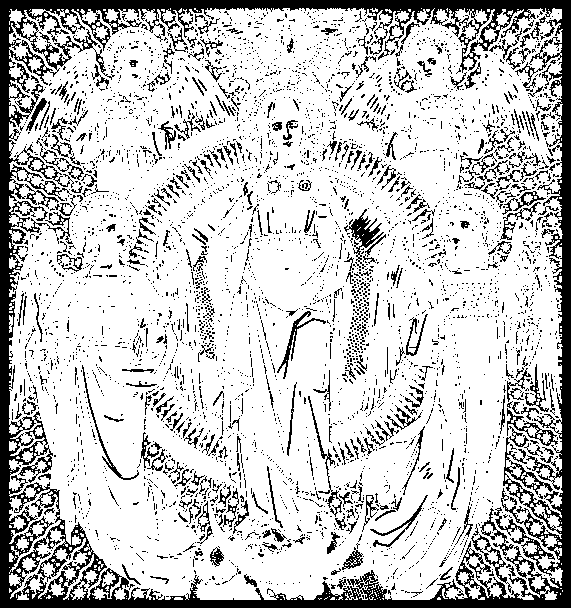
\includegraphics[width=0.44\textwidth]{../Images/Mary.pdf}
\end{center}
\vfill

%
% \newpage
%
% \begin{center}
%
%   \phantom{Ad maiorem Dei gloriam}
%
%   \vspace{0.5cm}
%
%   {\Huge\scshape\textls[150]{\MakeLowercase{Psalmodia}}}
%
%   \vspace{0.5cm}
%
%   {\Large\itshape Psalmody}
%
%   \vspace{0.5cm}
%
% \end{center}
%
% % This file is used as input to the main file.

\bisection{Post I Vesperas dominicæ et sollemnitatem}{After 1st Vespers of Sunday and Solemnities}\label{SundayI}

\bisubsectionnoline{Psalmus 4 \textemdash{} Gratiarum actio}{Psalm 4 \textemdash{} Thanksgiving}

\vspace{-0.1cm}

\bisentence{“Admirabilem fecit Dominus, quem suscitavit\\
a mortuis” \textup{(S. Augustinus).}}{“The Lord raised him from the dead and made him worthy\\
of all admiration” \textup{(St Augustine).}}

\bimusic{\gregorioscore{../AntiphonsAndPsalmsAndReadings/0Saturday/11229-an--miserere_mihi_domine--verona,H0C1.gabc}}{\GreColored{Ant. 1}\, Lord, have mercy and hear me.}

\bimusic[Vel, in tempore paschali:][Or, in Easter time:]{\gregorioscore{../AntiphonsAndPsalmsAndReadings/0Saturday/1942-an--alleluia._(t.p._ad_completorium)--solesmes_1961-no-signs.gabc}}{\GreColored{Ant.} Alleluia, alleluia, alleluia.}

\bireading{\gregorioscore{../AntiphonsAndPsalmsAndReadings/0Saturday/4-8G.gabc}}{\gregorioscore{../AntiphonsAndPsalmsAndReadings/0Saturday/4-8G-en.gabc}}

\verticalspacerpsalm

\bihangingpsalm{
miserére \textbf{me}i\redstar\\
et exáudi orati\textit{ónem} \textbf{me}am.

Fílii hóminum, úsquequo gravi \textbf{cor}de?\redstar\\
Ut quid dilígitis vanitátem et quǽri\textit{tis} \textit{men}\textbf{dá}cium?

Et scitóte quóniam mirificávit Dóminus sanctum \textbf{su}um;\redstar\\
Dóminus exáudiet, cum clamáve\textit{ro} \textit{ad} \textbf{e}um.

Irascímini et nolíte peccáre;\reddagger\\
loquímini in córdibus \textbf{ves}tris,\redstar\\
in cubílibus vestris et \textit{conqui}\textbf{é}scite.

Sacrificáte sacrifícium ius\textbf{tí}tiæ\redstar\\
et sperá\textit{te} \textit{in} \textbf{Dó}mino.

Multi dicunt:« Quis osténdit nobis \textbf{bo}na?».\redstar\\
Leva in signum super nos lumen vultus \textit{tui}, \textbf{Dó}mine!

Maiórem dedísti lætítiam in corde \textbf{me}o,\redstar\\
quam cum multiplicántur fruméntum et vi\textit{num} \textit{e}\textbf{ó}rum.

In pace in idípsum dórmiam et requi\textbf{és}cam,\redstar\\
quóniam tu, Dómine, singuláriter in spe con\textit{stitu}\textbf{ís}ti\mbox{ me.}

Glória Patri, et \textbf{Fí}lio,\redstar\\
et Spirí\textit{tui} \textbf{Sanc}to.

Sicut erat in princípio, et nunc, et \textbf{sem}per,\redstar\\
et in sǽcula sæcu\textit{lórum}. \textbf{A}men.
}
{
O men, how long will your \textbf{hearts} be closed,\redstar\\
will you love what is futile \textit{and seek} \textbf{what} is false?

It is the Lord who grants favours to those \textbf{whom} he\mbox{ loves;\redstar}\\
the Lord hears me whene\textit{ver I} \textbf{call} him.

Fear him; do not sin: ponder on your bed and \textbf{be} still\redstar\\
Make justice your sacrifice, \textit{and trust} \textbf{in} the Lord.

`What can bring us happiness?' \textbf{ma}ny say.\redstar\\
Let the light of your face \textit{shine on} \textbf{us}, O Lord.

You have put into my heart a \textbf{great}er joy\redstar\\
than they have from abundance of \textit{corn and} \textbf{new}\mbox{ wine.}

I will lie down in peace and sleep \textbf{comes} at once\redstar\\
for you alone, Lord, make me \textit{dwell in} \textbf{safe}ty.

Glory be to the Father and \textbf{to} the Son\redstar\\
and to the \textit{Holy} \textbf{Spi}rit,

as it was in the beginning, is now, and ever \textbf{shall} be,\redstar\\
world with\textit{out end}. \textbf{A}men.
}

\bimusic{\gregorioscore{../AntiphonsAndPsalmsAndReadings/0Saturday/11229-an--miserere_mihi_domine--verona,H0C1.gabc}}{\GreColored{Ant.} Lord, have mercy and hear me.}

\verticalspacer

\biinstruction{In tempore paschali, antiphona \textcolor{black}{Alleluia} dicitur tantum post \textcolor{black}{Psalmum 133} secundum antiphonam invenitur post lectionem brevem.}{In Easter time, the antiphon \textcolor{black}{Alleluia} is sung only after \textcolor{black}{Psalmum 133} conforming to the antiphon, which is found after the short reading.}

\bisubsection{Psalmus 133 \textemdash{} Vespertina oratio in templo (Extra Tempus Paschale)}{Psalm 133 \textemdash{} Evening prayer in the Temple (Outside Easter Time)}

\bisentence{“Laudem dicite Deo nostro, omnes servi eius et qui timetis eum,\\
pusilli et magni!” \textup{(Ap 19, 5).}}{“Praise our God, all you his servants, and all who revere him,\\
both great and small” \textup{(Ap 19:5).}}

\bimusic{\gregorioscore{../AntiphonsAndPsalmsAndReadings/0Saturday/11230-an--in_noctibus_benedicite--verona,H0C2.gabc}}{\GreColored{Ant. 2}\, Bless the Lord through the night.}

\bireading{\gregorioscore{../AntiphonsAndPsalmsAndReadings/0Saturday/134-D_d.gabc}}{\gregorioscore{../AntiphonsAndPsalmsAndReadings/0Saturday/134-D_d-en.gabc}}

\verticalspacerpsalm

\bihangingpsalm{
Extóllite manus vestras ad \textit{sanctu}\textbf{á}rium\redstar\\
et bene\textit{díci}\textit{te} \textbf{Dó}minum.

Benedícat te Dómi\textit{nus} \textit{ex} \textbf{Si}on,\redstar\\
qui fecit \textit{cælum} \textit{et} \textbf{ter}ram.

Glória Pa\textit{tri}, \textit{et} \textbf{Fí}lio,\redstar\\
et Spi\textit{rítu}\textit{i} \textbf{Sanc}to.

Sicut erat in princípio, et \textit{nunc}, \textit{et} \textbf{sem}per,\redstar\\
et in sǽcula sæ\textit{culó}\textit{rum}. \textbf{A}men.
}
{
Lift up your hands \textit{to the} \textbf{ho}ly place\redstar\\
and \textit{bless the Lord} \textbf{through} the night.

May the Lord bless \textit{you from} \textbf{Si}on,\redstar\\
he who made \textit{both heaven} \textbf{and} earth.

Glory be to the Fath\textit{er and} \textbf{to} the Son\redstar\\
and to \textit{the Holy} \textbf{Spi}rit,

As it was in the beginning, is now, and \textit{ever} \textbf{shall} be,\redstar\\
world \textit{without end}. \textbf{A}men.
}

\bimusic{\gregorioscore{../AntiphonsAndPsalmsAndReadings/0Saturday/11230-an--in_noctibus_benedicite--verona,H0C2.gabc}}{\GreColored{Ant.} Bless the Lord through the night.}

\vspace{-0.1cm}
\bisubsection{Lectio brevis \textemdash{} Deut 6, 4-7}{Short reading \textemdash{} Deut 6:4-7}
\vspace{-0.1cm}

\bireading{\gregorioscore{../AntiphonsAndPsalmsAndReadings/0Saturday/SaturdayLectioBrevis.gabc}}{\gregorioscore{../AntiphonsAndPsalmsAndReadings/0Saturday/SaturdayLectioBrevis-en.gabc}}

\vspace{0.1cm}

\biinstruction{Responsorium breve subsequitur, p. \textcolor{black}{\pageref{ResponsoriumBreve}.}}{The short response follows, p. \textcolor{black}{\pageref{ResponsoriumBreve}.}}

\redlineseparator

\bisubsection{Psalmus 133 \textemdash{} Vespertina oratio in templo (Tempus Paschale)}{Psalm 133 \textemdash{} Evening prayer in the Temple (Easter Time)}

\bisentence{“Laudem dicite Deo nostro, omnes servi eius et qui timetis eum,\\
pusilli et magni!” \textup{(Ap 19, 5).}}{“Praise our God, all you his servants, and all who revere him,\\
both great and small” \textup{(Ap 19:5).}}

\bireading{\gregorioscore{../AntiphonsAndPsalmsAndReadings/0Saturday/134-8G.gabc}}{\gregorioscore{../AntiphonsAndPsalmsAndReadings/0Saturday/134-8G-en.gabc}}

\verticalspacerpsalm

\bihangingpsalm{
Extóllite manus vestras ad sanctu\textbf{á}rium\redstar\\
et benedí\textit{cite} \textbf{Dó}minum.

Benedícat te Dóminus ex \textbf{Si}on,\redstar\\
qui fecit cæ\textit{lum} \textit{et} \textbf{ter}ram.

Glória Patri, et \textbf{Fí}lio,\redstar\\
et Spirí\textit{tui} \textbf{Sanc}to.

Sicut erat in princípio, et nunc, et \textbf{sem}per,\redstar\\
et in sǽcula sæcu\textit{lórum}. \textbf{A}men.
}
{
Lift up your hands to the \textbf{ho}ly place\redstar\\
and bless \textit{the Lord} \textbf{through} the night.

May the Lord bless you from \textbf{Si}on,\redstar\\
he who made both \textit{heaven} \textbf{and} earth.

Glory be to the Father and \textbf{to} the Son\redstar\\
and to the \textit{Holy} \textbf{Spi}rit,

As it was in the beginning, is now, and ever \textbf{shall} be,\redstar\\
world with\textit{out end}. \textbf{A}men.
}

\bimusic{\gregorioscore{../AntiphonsAndPsalmsAndReadings/0Saturday/1942-an--alleluia._(t.p._ad_completorium)--solesmes_1961-no-signs.gabc}}{\GreColored{Ant.} Alleluia, alleluia, alleluia.}

\vfill
\begin{center}
  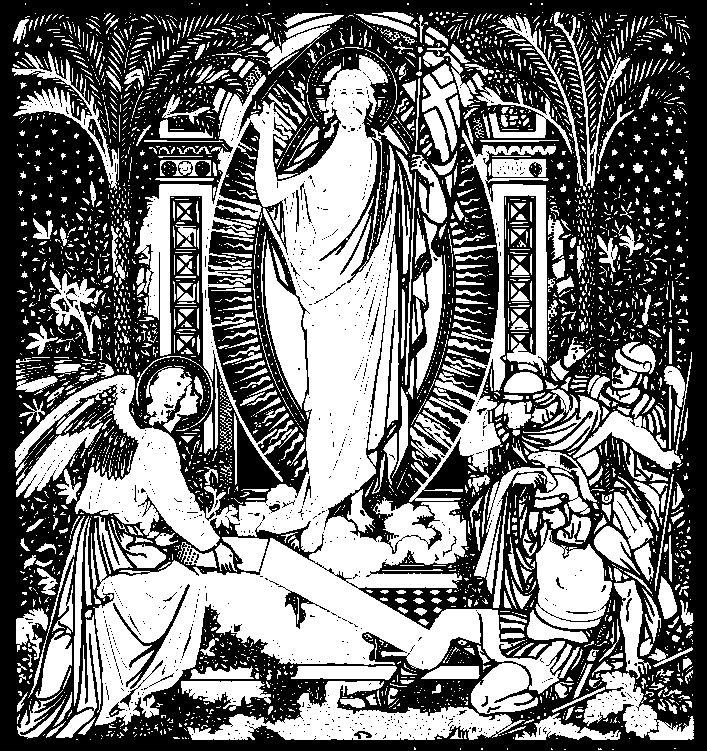
\includegraphics[width=0.44\textwidth]{../Images/Resurrection.pdf}
\end{center}
\vfill

%
% % This file is used as input to the main file.

% \newpage
\newgeometry{left=1cm, right=1cm, top=1cm, bottom=1.0cm}
\thispagestyle{empty} % Custom number

\bisection{Post II Vesperas dominicæ et sollemnitatem}{\vspace{-0.1cm}After 2nd Vespers of Sunday and Sollemnities}\label{SundayII}

\vspace{-0.1cm}
\bisubsectionnoline{Psalmus 90 \textemdash{} In protectione Altissimi}{Psalm 90 \textemdash{} In the shelter of the Most High}
\vspace{-0.1cm}

\bisentence{“Ecce dedi vobis potestatem calcandi supra\\
serpentes et scorpiones” \textup{(Lc 10, 19).}}{“Behold, I have given you power to tread under foot both\\
serpents and scorpions” \textup{(Lk 10:19).}}
\vspace{-0.1cm}

\bimusic{\gregorioscore{../AntiphonsAndPsalmsAndReadings/1Sunday/11232-an--qui_habitat_in--verona,H1C1.gabc}}{\GreColored{Ant.} He that dwells in the aid of the most High, shall abide under the protection of the God of heaven.}

\vspace{-0.1cm}
\bimusic[Vel, in tempore paschali:\vspace{-0.1cm}][Or, in Easter time:\vspace{-0.1cm}]{\gregorioscore{../AntiphonsAndPsalmsAndReadings/1Sunday/AlleluiaQuaSu2-no-signs.gabc}}{\GreColored{Ant.} Alleluia, alleluia, alleluia, alleluia.}

\bireading{\gregorioscore{../AntiphonsAndPsalmsAndReadings/1Sunday/91-8G.gabc}}{\gregorioscore{../AntiphonsAndPsalmsAndReadings/1Sunday/91-8G-en.gabc}}

\verticalspacerpsalm
\vspace{-0.05cm}

\bihangingpsalm{Dicet Dómino:~\GreColored{†}\\
« Refúgium meum et fortitúdo \textbf{me}a,~\GreColored{*}\\
Deus meus, sperá\textit{bo} \textit{in} \textbf{e}um».

Quóniam ipse liberábit te de láqueo ve\textbf{nán}tium~\GreColored{*}\\
et a ver\textit{bo} \textit{ma}\textbf{lí}gno.

Alis suis obumbrábit tibi,~\GreColored{†}\\
et sub pennas eius con\textbf{fú}gies;~\GreColored{*}\\
scutum et loríca vé\textit{ritas} \textbf{e}ius.

Non timébis a timóre noctúrno, a sagítta volánte in die,~\GreColored{†}\\
6 a peste perambulánte in \textbf{té}nebris,~\GreColored{*}\\
ab extermínio vastánte \textit{in} \textit{me}\textbf{rí}die.

Cadent a látere tuo mille~\GreColored{†}\\
et decem mília a dextris \textbf{tu}is;~\GreColored{*}\\
ad te autem non ap\textit{propin}\textbf{quá}bit.

Verúmtamen óculis tuis conside\textbf{rá}bis,~\GreColored{*}\\
et retributiónem peccató\textit{rum} \textit{vi}\textbf{dé}bis.

Quóniam tu es, Dómine, refúgium \textbf{me}um.~\GreColored{*}\\
Altíssimum posuísti habitá\textit{culum} \textbf{tu}um.

Non accédet ad te \textbf{ma}lum,~\GreColored{*}\\
et flagéllum non appropinquábit taberná\textit{culo} \textbf{tu}o,

quóniam ángelis suis mandábit \textbf{de} te,~\GreColored{*}\\
ut custódiant te in ómnibus \textit{viis} \textbf{tu}is.

In mánibus por\textbf{tá}bunt te,~\GreColored{*}\\
ne forte offéndas ad lápidem \textit{pedem} \textbf{tu}um.

Super áspidem et basilíscum ambu\textbf{lá}bis~\GreColored{*}\\
et conculcábis leónem \textit{et} \textit{dra}\textbf{có}nem.

Quóniam mihi adhǽsit, liberábo \textbf{e}um;~\GreColored{*}\\
suscípiam eum, quóniam cognóvit \textit{nomen} \textbf{me}um.

Clamábit ad me, et ego exáudiam eum;~\GreColored{†}\\
cum ipso sum in tribulati\textbf{ó}ne;~\GreColored{*}\\
erípiam eum et glorifi\textit{cábo} \textbf{e}um.

Longitúdine diérum replébo \textbf{e}um~\GreColored{*}\\
et osténdam illi salu\textit{táre} \textbf{me}um.

Glória Patri, et \textbf{Fí}lio,~\GreColored{*}\\
et Spirí\textit{tui} \textbf{Sanc}to.

Sicut erat in princípio, et nunc, et \textbf{sem}per,~\GreColored{*}\\
et in sǽcula sæcu\textit{lórum}. \textbf{A}men.}
{
Says to the Lord: `My \textbf{re}fuge,~\GreColored{*}\\
my stronghold, my \textit{God in} \textbf{whom} I trust!'

It is he who will free you \textbf{from} the snare~\GreColored{*}\\
of the fowler who seeks \textit{to des}\textbf{troy} you;

He will conceal you with his \textbf{pin}ions~\GreColored{*}\\
and under his wings you \textit{will find} \textbf{re}fuge.

You will not fear the terror \textbf{of} the night~\GreColored{*}\\
nor the ar\textit{row that} \textbf{flies} by day,

Nor the plague that prowls in the \textbf{dark}ness~\GreColored{*}\\
nor the scourge \textit{that lays} \textbf{waste} at noon.

A thousand may fall \textbf{at} your side,~\GreColored{*}\\
ten thousand \textit{fall at} \textbf{your} right,

You, it will never \textbf{ap}proach;~\GreColored{*}\\
his faithfulness is \textit{buckler} \textbf{and} shield.

Your eyes have only \textbf{to} look~\GreColored{*}\\
to see how the wi\textit{cked are} \textbf{re}paid,

You who have said: `Lord, my \textbf{re}fuge!'~\GreColored{*}\\
and have made the Most \textit{High your} \textbf{dwell}ing.

Upon you no evil \textbf{shall} fall,~\GreColored{*}\\
no plague \textit{approach} \textbf{where} you dwell.

For you has he commanded his \textbf{an}gels,~\GreColored{*}\\
to keep \textit{you in} \textbf{all} your ways.

They shall bear you u\textbf{pon} their hands~\GreColored{*}\\
lest you strike your \textit{foot a}\textbf{gainst} a stone.

On the lion and the viper \textbf{you} will tread~\GreColored{*}\\
and trample the young lion \textit{and the} \textbf{dra}gon.

Since he clings to me in love, I will \textbf{free} him;~\GreColored{*}\\
protect him \textit{for he} \textbf{knows} my name.

When he calls I shall answer: `I am \textbf{with} you,'~\GreColored{*}\\
I will save him in distress and \textit{give him} \textbf{glo}ry.

With length of life I will con\textbf{tent} him;~\GreColored{*}\\
I shall let him see my \textit{saving} \textbf{pow}er.

Glory be to the Father and \textbf{to} the Son~\GreColored{*}\\
and to the \textit{Holy} \textbf{Spi}rit,

As it was in the beginning, is now, and ever \textbf{shall} be,~\GreColored{*}\\
world with\textit{out end}. \textbf{A}men.
}

\vspace{-0.2cm}
\begin{center}
  17
\end{center}
\restoregeometry

\bimusic{\gregorioscore{../AntiphonsAndPsalmsAndReadings/1Sunday/11232-an--qui_habitat_in--verona,H1C1.gabc}}{\GreColored{Ant.} He that dwells in the aid of the most High, shall abide under the protection of the God of heaven.}

\bisubsection{Lectio brevis \textemdash{} Ap 22, 4. 5}{Short reading \textemdash{} Ap 22:4-5}

\bireading{\gregorioscore{../AntiphonsAndPsalmsAndReadings/1Sunday/SundayLectioBrevis.gabc}}{\gregorioscore{../AntiphonsAndPsalmsAndReadings/1Sunday/SundayLectioBrevis-en.gabc}}

\verticalspacer

\biinstruction{Responsorium breve subsequitur, p. \textcolor{black}{\pageref{ResponsoriumBreve}.}}{The short response follows, p. \textcolor{black}{\pageref{ResponsoriumBreve}.}}

%
% % This file is used as input to the main file.

\bisection{Feria Secunda}{Monday}\label{Monday}

\bisubsection{Psalmus 85 \textemdash{} Pauperis in rebus adversis oratio}{Psalm 85 \textemdash{} A poor man's prayer in time of trouble}

\bisentence{“Benedictus Deus, qui consolatur nos in omni\\
tribulatione nostra” \textup{(2 Cor 1, 3. 4).}}{“Blessed be God, who comforts us in all\\
our sorrows” \textup{(2 Cor 1:3-4).}}

\bimusic{\gregorioscore{../AntiphonsAndPsalmsAndReadings/2Monday/11233-an--intende_voci_orationis--verona,H2C1.gabc}}{\GreColored{Ant.} Attend to the sound of my prayer.}

\bimusic[Vel, in tempore paschali:][Or, in Easter time:]{\gregorioscore{../AntiphonsAndPsalmsAndReadings/2Monday/10164-an--alleluia_(tuesday_p._t._at_lauds)---no-signs.gabc}}{\GreColored{Ant.} Alleluia, alleluia, alleluia.}

\bireading{\gregorioscore{../AntiphonsAndPsalmsAndReadings/2Monday/86-8G.gabc}}{\gregorioscore{../AntiphonsAndPsalmsAndReadings/2Monday/86-8G-en.gabc}}

\verticalspacerpsalm

\bihangingpsalm{
Custódi ánimam meam, quóniam \textbf{sanc}tus sum;~*\\
salvum fac servum tuum, Deus meus, spe\textit{rántem} \textbf{in} te.

Miserére mei, \textbf{Dó}mine,~*\\
quóniam ad te clamávi \textit{tota} \textbf{di}e.

Lætífica ánimam servi \textbf{tu}i,~*\\
quóniam ad te, Dómine, ánimam me\textit{am} \textit{le}\textbf{vá}vi.

Quóniam tu, Dómine, suávis et \textbf{mi}tis~*\\
et multæ misericórdiæ ómnibus invo\textit{cánti}\textbf{bus} te.

Auribus pércipe, Dómine, oratiónem \textbf{me}am~*\\
et inténde voci deprecati\textit{ónis} \textbf{me}æ.

In die tribulatiónis meæ clamávi \textbf{ad} te,~*\\
quia ex\textit{áudi}\textbf{es} me.

Non est símilis tui in diis, \textbf{Dó}mine,~*\\
et nihil sicut ó\textit{pera} \textbf{tu}a.

Omnes gentes, quascúmque fecísti, vénient~†\\
et adorábunt coram te, \textbf{Dó}mine,~*\\
et glorificábunt \textit{nomen} \textbf{tu}um,

quóniam magnus es tu et fáciens mira\textbf{bí}lia:~*\\
tu es \textit{Deus} \textbf{so}lus.

Doce me, Dómine, viam \textbf{tu}am,~*\\
et ingrédiar in veri\textit{táte} \textbf{tu}a;

simplex fac cor \textbf{me}um,~*\\
ut tímeat \textit{nomen} \textbf{tu}um.

Confitébor tibi, Dómine Deus meus, in toto corde \textbf{me}o~*\\
et glorificábo nomen tuum \textit{in} \textit{æ}\textbf{tér}num,

quia misericórdia tua magna est \textbf{su}per me,~*\\
et eruísti ánimam meam ex inférno in\textit{feri}\textbf{ó}ri.

Deus, supérbi insurrexérunt super me,~†\\
et synagóga poténtium quæsiérunt ánimam \textbf{me}am,~*\\
et non proposuérunt te in con\textit{spéctu} \textbf{su}o.

Et tu, Dómine, Deus miserátor et mi\textbf{sé}ricors,~*\\
pátiens et multæ misericórdiæ et \textit{veri}\textbf{tá}tis,

réspice in me et miserére mei;~†\\
da fortitúdinem tuam púero \textbf{tu}o~*\\
et salvum fac fílium an\textit{cíllæ} \textbf{tu}æ.

Fac mecum signum in bonum,~†\\
ut vídeant, qui odérunt me, et confun\textbf{dán}tur,~*\\
quóniam tu, Dómine, adiuvísti me et conso\textit{látus} \textbf{es} me.

Glória Patri, et \textbf{Fí}lio,~*\\
et Spirí\textit{tui} \textbf{Sanc}to.

Sicut erat in princípio, et nunc, et \textbf{sem}per,~*\\
et in sǽcula sæcu\textit{lórum}. \textbf{A}men.
}
{
Preserve my life, for I am \textbf{faith}ful;~*\\
save the ser\textit{vant who} \textbf{trusts} in you.

You are my God, have mercy \textbf{on} me, Lord,~*\\
for I cry to you \textit{all the} \textbf{day} long.

Give joy to your servant, \textbf{O} Lord,~*\\
for to you I \textit{lift up} \textbf{my} soul.

O Lord, you are good and for\textbf{giv}ing,~*\\
full of \textit{love to} \textbf{all} who call.

Give heed, O Lord, \textbf{to} my prayer~*\\
and attend to the \textit{sound of} \textbf{my} voice.

In the day of distress \textbf{I} will call~*\\
and sure\textit{ly you} \textbf{will} reply.

Among the gods there is none like \textbf{you}, O Lord;~*\\
nor work \textit{to com\textbf{}pare} with yours.

All the nations shall come to ad\textbf{ore} you~*\\
and glori\textit{fy your} \textbf{name}, O Lord:

for you are great and do marvel\textbf{lous} deeds,~*\\
you \textit{who al\textbf{}one} are God.

Show me, Lord, your way~†\\
so that I may walk \textbf{in} your truth.~*\\
Guide my \textit{heart to} \textbf{fear} your name.

I will praise you, Lord my God, with \textbf{all} my heart~*\\
and glorify your \textit{name for} \textbf{ev}er;

for your love to me \textbf{has} been great:~*\\
you have saved me from the \textit{depths of} \textbf{the} grave.

The proud have risen against me;~†\\
ruthless men \textbf{seek} my life;~*\\
to \textit{you they} \textbf{pay} no heed.

But you, God of mercy and com\textbf{pas}sion,~*\\
slow to \textit{anger}, \textbf{O} Lord,

abounding in \textbf{love} and truth,~*\\
turn and take \textit{pity} \textbf{on} me.

O give your strength to your \textbf{ser}vant~*\\
and \textit{save your} \textbf{hand}maid’s son.

Show me a sign of your favour~†\\
that my foes may see \textbf{to} their shame~*\\
that you console me and \textit{give me} \textbf{your} help.

Glory be to the Father and \textbf{to} the Son~*\\
and to the \textit{Holy} \textbf{Spi}rit,

as it was in the beginning, is now, and ever \textbf{shall} be,~*\\
world with\textit{out end}. \textbf{A}men.
}

\bimusic{\gregorioscore{../AntiphonsAndPsalmsAndReadings/2Monday/11233-an--intende_voci_orationis--verona,H2C1.gabc}}{\GreColored{Ant.} Attend to the sound of my prayer.}

\bimusic[Vel, in tempore paschali:][Or, in Easter time:]{\gregorioscore{../AntiphonsAndPsalmsAndReadings/2Monday/10164-an--alleluia_(tuesday_p._t._at_lauds)---no-signs.gabc}}{\GreColored{Ant.} Alleluia, alleluia, alleluia.}

\bisubsection{Lectio brevis \textemdash{} 1 Th 5, 9. 10}{Short reading \textemdash{} 1 Th 5:9-10}

\bireading{\gregorioscore{../AntiphonsAndPsalmsAndReadings/2Monday/MondayLectioBrevis.gabc}}{\gregorioscore{../AntiphonsAndPsalmsAndReadings/2Monday/MondayLectioBrevis-en.gabc}}

\verticalspacer

\biinstruction{Responsorium breve subsequitur, p. \textcolor{black}{\pageref{ResponsoriumBreve}.}}{The short response follows, p. \textcolor{black}{\pageref{ResponsoriumBreve}.}}

%
% % This file is used as input to the main file.

\newpage

\bisection{Feria Tertia}{Tuesday}\label{Tuesday}

\bisubsectionnoline{Psalmus 142, 1-11 \textemdash{} In angustiis oratio}{Psalm 142:1-11 \textemdash{} A prayer in time of trouble}

\bisentence{“Non iustificatur homo ex operibus legis nisi\\
per fidem Iesu Christi” \textup{(Gal 2, 16).}}{“A man is made righteous not by obedience to the Law, but\\
by faith in Jesus Christ” \textup{(Gal 2:16).}}

\bimusic{\gregorioscore{../AntiphonsAndPsalmsAndReadings/3Tuesday/11234-an--ne_intres_in--verona,H3C1.gabc}}{\GreColored{Ant.} Enter not into judgment with your servant.}

\bimusic[Vel, in tempore paschali:][Or, in Easter time:]{\gregorioscore{../AntiphonsAndPsalmsAndReadings/3Tuesday/10442-an--alleluia_(dominica_per_annum_ad_laudes)--solesmes_1934-no-signs.gabc}}{\GreColored{Ant.} Alleluia, alleluia, alleluia.}

\bireading{\gregorioscore{../AntiphonsAndPsalmsAndReadings/3Tuesday/143-8G.gabc}}{\gregorioscore{../AntiphonsAndPsalmsAndReadings/3Tuesday/143-8G-en.gabc}}

\verticalspacerpsalm

\bihangingpsalm{
Et non intres in iudícium cum servo \textbf{tu}o,\redstar\\
quia non iustificábitur in conspéctu tuo \textit{omnis} \textbf{vi}vens.

Quia persecútus est inimícus ánimam meam,\reddagger\\
contrívit in terra vitam \textbf{me}am,\redstar\\
collocávit me in obscúris sicut mórtu\textit{os} \textit{a} \textbf{sǽ}culo.

Et anxiátus est in me spíritus \textbf{me}us,\redstar\\
in médio mei obrígu\textit{it} \textit{cor} \textbf{me}um.

Memor fui diérum antiquórum,\reddagger\\
meditátus sum in ómnibus opéribus \textbf{tu}is,\redstar\\
in factis mánuum tuárum re\textit{cogi}\textbf{tá}bam.

Expándi manus meas \textbf{ad} te,\redstar\\
ánima mea sicut terra sine \textit{aqua} \textbf{ti}bi.

Velóciter exáudi me, \textbf{Dó}mine;\redstar\\
defécit spí\textit{ritus} \textbf{me}us.

Non abscóndas fáciem tuam \textbf{a} me,\redstar\\
ne símilis fiam descendénti\textit{bus} \textit{in} \textbf{la}cum.

Audítam fac mihi mane misericórdiam \textbf{tu}am,\redstar\\
quia in \textit{te} \textit{spe}\textbf{rá}vi.

Notam fac mihi viam, in qua \textbf{ám}bulem,\redstar\\
quia ad te levávi á\textit{nimam} \textbf{me}am.

Eripe me de inimícis \textbf{me}is,\redstar\\
Dómine, ad \textit{te} \textit{con}\textbf{fú}gi.

Doce me fácere voluntátem \textbf{tu}am,\redstar\\
quia Deus \textit{meus} \textbf{es} tu.

Spíritus tuus bonus dedúcet me in terram \textbf{rec}tam;\redstar\\
propter nomen tuum, Dómine, vi\textit{vifi}\textbf{cá}bis me.

In iustítia tua edúces de tribulatióne ánimam \textbf{me}am\redstar\\
et in misericórdia tua dispérdes ini\textit{mícos} \textbf{me}os;

et perdes omnes, qui tríbulant ánimam \textbf{me}am,\redstar\\
quóniam ego \textit{servus} \textbf{tu}us sum.

Glória Patri, et \textbf{Fí}lio,\redstar\\
et Spirí\textit{tui} \textbf{Sanc}to.

Sicut erat in princípio, et nunc, et \textbf{sem}per,\redstar\\
et in sǽcula sæcu\textit{lórum}. \textbf{A}men.
}
{
Do not call your servant to \textbf{judge}ment\redstar\\
for no one is \textit{just in} \textbf{your} sight.

The enemy pur\textbf{sues} my soul;\redstar\\
he has crushed \textit{my life} \textbf{to} the ground;

he has made me dwell in \textbf{dark}ness\redstar\\
like the dead, \textit{long for}\textbf{got}ten.

Therefore my \textbf{spi}rit fails;\redstar\\
my heart is \textit{numb with}\textbf{in} me.

I remember the days \textbf{that} are past:\redstar\\
I \textit{ponder} \textbf{all} your works.

I muse on what your hand has wrought\reddagger\\
and to you I stretch \textbf{out} my hands.\redstar\\
Like a parched land \textit{my soul} \textbf{thirsts} for you.

Lord, make haste and \textbf{an}swer;\redstar\\
for my spirit \textit{fails with}\textbf{in} me.

Do not \textbf{hide} your face\redstar\\
lest I become \textit{like those} \textbf{in} the grave.

In the morning let me \textbf{know} your love\redstar\\
for I \textit{put my} \textbf{trust} in you.

Make me know the way \textbf{I} should walk:\redstar\\
to you \textit{I lift} \textbf{up} my soul.

Rescue me, Lord, from my \textbf{en}emies;\redstar\\
I have fled to \textit{you for} \textbf{re}fuge.

Teach me to do \textbf{your} will\redstar\\
for you, \textit{O Lord}, \textbf{are} my God.

Let your good spirit \textbf{guide} me\redstar\\
in ways that are \textit{level} \textbf{and} smooth.

For your name’s sake, Lord, \textbf{save} my life;\redstar\\
in your justice save my \textit{soul from} \textbf{dis}tress.

Glory be to the Father and \textbf{to} the Son\redstar\\
and to the \textit{Holy} \textbf{Spi}rit,

as it was in the beginning, is now, and ever \textbf{shall} be,\redstar\\
world with\textit{out end}. \textbf{A}men.
}

\bimusic{\gregorioscore{../AntiphonsAndPsalmsAndReadings/3Tuesday/11234-an--ne_intres_in--verona,H3C1.gabc}}{\GreColored{Ant.} Enter not into judgment with your servant.}

\bimusic[Vel, in tempore paschali:][Or, in Easter time:]{\gregorioscore{../AntiphonsAndPsalmsAndReadings/3Tuesday/10442-an--alleluia_(dominica_per_annum_ad_laudes)--solesmes_1934-no-signs.gabc}}{\GreColored{Ant.} Alleluia, alleluia, alleluia.}

\vspace{-0.1cm}
\bisubsection{Lectio brevis \textemdash{} 1 Petr 5, 8. 9}{Short reading \textemdash{} 1 Pet 5:8-9}
\vspace{-0.1cm}

\bireading{\gregorioscore{../AntiphonsAndPsalmsAndReadings/3Tuesday/TuesdayLectioBrevis.gabc}}{\gregorioscore{../AntiphonsAndPsalmsAndReadings/3Tuesday/TuesdayLectioBrevis-en.gabc}}

\verticalspacer

\biinstruction{Responsorium breve subsequitur, p. \textcolor{black}{\pageref{ResponsoriumBreve}.}}{The short response follows, p. \textcolor{black}{\pageref{ResponsoriumBreve}.}}

%
% % This file is used as input to the main file.

\vspace{-0.1cm}
\bisection{Feria Quarta}{Wednesday}\label{Wednesday}

\vspace{-0.1cm}
\bisubsection{Psalmus 30, 2-6 \textemdash{} Afflicti supplicatio cum fiducia}{Psalm 30:2-6 \textemdash{} Trustful prayer in time of adversity}
\vspace{-0.1cm}

\bisentence{“Pater, in manus tuas commendo spiritum meum” \textup{(Lc 23, 46).}}{“Father, into your hands I commend my spirit” \textup{(Lk 23:46).}}

\bimusic{\gregorioscore{../AntiphonsAndPsalmsAndReadings/4Wednesday/11235-an--esto_mihi_domine--verona,H4C1.gabc}}{\GreColored{Ant. 1}\, O God, be my protector and my refuge.}

\bimusic[Vel, in tempore paschali:][Or, in Easter time:]{\gregorioscore{../AntiphonsAndPsalmsAndReadings/4Wednesday/8751-an--alleluia_(monday_p._t._at_lauds)_--solesmes_1934-no-signs.gabc}}{\GreColored{Ant.} Alleluia, alleluia, alleluia.}

\bireading{\gregorioscore{../AntiphonsAndPsalmsAndReadings/4Wednesday/31-6.gabc}}{\gregorioscore{../AntiphonsAndPsalmsAndReadings/4Wednesday/31-6-en.gabc}}

\verticalspacerpsalm

\bihangingpsalm{
Inclína ad me au\textit{rem} \textbf{tu}am,~*\\
accélera, ut \textit{é}\textit{ru}\textbf{as} me.

Esto mihi in rupem præsídii et in domum \textit{mu}\textbf{ní}tam,~*\\
ut sal\textit{vum} \textit{me} \textbf{fá}cias.

Quóniam fortitúdo mea et refúgium me\textit{um} \textbf{es} tu~*\\
et propter nomen tuum dedúces \textit{me} \textit{et} \textbf{pa}sces me.

Edúces me de láqueo, quem abscondé\textit{runt} \textbf{mi}hi,~*\\
quóniam tu es forti\textit{tú}\textit{do} \textbf{me}a.

In manus tuas comméndo spíri\textit{tum} \textbf{me}um;~*\\
redemísti me, Dómine, Deus \textit{ve}\textit{ri}\textbf{tá}tis.

Glória Patri, \textit{et} \textbf{Fí}lio,~*\\
et Spirí\textit{tu}\textit{i} \textbf{Sanc}to.

Sicut erat in princípio, et nunc, \textit{et} \textbf{sem}per,~*\\
et in sǽcula sæcu\textit{ló}\textit{rum}. \textbf{A}men.
}
{
In your just\textit{ice}, \textbf{set} me free,~*\\
hear me and speed\textit{ily} \textbf{res}cue me.

Be a rock of re\textit{fuge} \textbf{for} me,~*\\
a mighty strong\textit{hold to} \textbf{save} me,

for you are my rock, \textit{my} \textbf{strong}hold.~*\\
For your name’s sake, lead \textit{me and} \textbf{guide} me.

Release me from the snares they \textit{have} \textbf{hid}den~*\\
for you \textit{are my} \textbf{re}fuge, Lord.

Into your hands I commend \textit{my} \textbf{spi}rit.~*\\
It is you who will \textit{redeem} \textbf{me}, Lord.

Glory be to the Father \textit{and} \textbf{to} the Son~*\\
and to the \textit{Holy} \textbf{Spi}rit,

as it was in the beginning, is now, and ev\textit{er} \textbf{shall} be,~*\\
world with\textit{out end}. \textbf{A}men.
}

\bimusic{\gregorioscore{../AntiphonsAndPsalmsAndReadings/4Wednesday/11235-an--esto_mihi_domine--verona,H4C1.gabc}}{\GreColored{Ant.} O God, be my protector and my refuge.}

\verticalspacer

\vspace{-0.15cm}
\biinstruction{In tempore paschali, antiphona \textcolor{black}{Alleluia} dicitur tantum post \textcolor{black}{Psalmum 129} secundum antiphonam invenitur post lectionem brevem.}{In Easter time, the antiphon \textcolor{black}{Alleluia} is sung only after \textcolor{black}{Psalmum 129} conforming to the antiphon, which is found after the short reading.}
\vspace{-0.30cm}

\bisubsection{Psalmus 129 \textemdash{} De profundis clamavi}{Psalm 129 \textemdash{} Out of the depths}
\vspace{-0.20cm}

\bisentence{“Ipse salvum faciet populum suum a peccatis eorum” \textup{(Mt 1, 21).}}{“He will save his people from their sins” \textup{(Mt 1:21).}}

\bimusic{\gregorioscore{../AntiphonsAndPsalmsAndReadings/4Wednesday/11236-an--de_profundis_clamavi--verona,H4C2.gabc}}{\GreColored{Ant. 2}\, Out of the depths I cry to you, O Lord.}

\bireading{\gregorioscore{../AntiphonsAndPsalmsAndReadings/4Wednesday/130-8G.gabc}}{\gregorioscore{../AntiphonsAndPsalmsAndReadings/4Wednesday/130-8G-en.gabc}}

\verticalspacerpsalm

\bihangingpsalm{
Fiant aures tuæ inten\textbf{dén}tes~*\\
in vocem deprecati\textit{ó}\textit{nis} \textbf{me}æ.

Si iniquitátes observáveris, \textbf{Dó}mine,~*\\
Dómine, quis \textit{sus}\textit{ti}\textbf{né}bit?

Quia apud te propitiáti\textbf{o} est,~*\\
ut \textit{ti}\textit{me}\textbf{á}mus te.

Sustínui te, \textbf{Dó}mine,~*\\
sustínuit ánima mea in \textit{ver}\textit{bo} \textbf{e}ius;

sperávit ánima mea in \textbf{Dó}mino~*\\
magis quam custó\textit{des} \textit{au}\textbf{ró}ram.

Magis quam custódes au\textbf{ró}ram~*\\
speret Isra\textit{ël} \textit{in} \textbf{Dó}mino,

quia apud Dóminum miseri\textbf{cór}dia,~*\\
et copiósa apud e\textit{um} \textit{red}\textbf{émp}tio.

Et ipse rédimet \textbf{Is}raël~*\\
ex ómnibus iniquitá\textit{ti}\textit{bus} \textbf{e}ius.

Glória Patri, et \textbf{Fí}lio,~*\\
et Spirí\textit{tu}\textit{i} \textbf{Sanc}to.

Sicut erat in princípio, et nunc, et \textbf{sem}per,~*\\
et in sǽcula sæcu\textit{ló}\textit{rum}. \textbf{A}men.
}
{
If you, O Lord, should \textbf{mark} our guilt,~*\\
\textit{Lord, who} \textbf{would} survive?

But with you is found for\textbf{give}ness:~*\\
for this \textit{we re}\textbf{vere} you.

My soul is waiting \textbf{for} the Lord.~*\\
I \textit{count} on \textbf{his} word.

My soul is longing \textbf{for} the Lord~*\\
more than watch\textit{man for} \textbf{day}break.

Let the watchman count on \textbf{day}break~*\\
and \textit{Israel} \textbf{on} the Lord.

Because with the Lord there is \textbf{mer}cy~*\\
and fullness \textit{of re}\textbf{demp}tion,

Israel indeed he \textbf{will} redeem~*\\
from all \textit{its in}\textbf{i}quity.

Glory be to the Father and \textbf{to} the Son~*\\
and to the \textit{Holy} \textbf{Spi}rit,

as it was in the beginning, is now, and ever \textbf{shall} be,~*\\
world with\textit{out end}. \textbf{A}men.
}

\bimusic{\gregorioscore{../AntiphonsAndPsalmsAndReadings/4Wednesday/11236-an--de_profundis_clamavi--verona,H4C2.gabc}}{\GreColored{Ant.} Out of the depths I cry to you, O Lord.}

\bisubsection{Lectio brevis \textemdash{} Eph 4, 26. 27}{Short reading \textemdash{} Eph 4:26-27}

\bireading{\gregorioscore{../AntiphonsAndPsalmsAndReadings/4Wednesday/WednesdayLectioBrevis.gabc}}{\gregorioscore{../AntiphonsAndPsalmsAndReadings/4Wednesday/WednesdayLectioBrevis-en.gabc}}

\verticalspacer

\biinstruction{Responsorium breve subsequitur, p. \textcolor{black}{\pageref{ResponsoriumBreve}.}}{The short response follows, p. \textcolor{black}{\pageref{ResponsoriumBreve}.}}

% \redlineseparator

\bisubsection{Psalmus 129 \textemdash{} De profundis clamavi (t. p.)}{Psalm 129 \textemdash{} Out of the depths (E. T.)}

\bisentence{“Ipse salvum faciet populum suum a peccatis eorum” \textup{(Mt 1, 21).}}{“He will save his people from their sins” \textup{(Mt 1:21).}}

\bireading{\gregorioscore{../AntiphonsAndPsalmsAndReadings/4Wednesday/130-6.gabc}}{\gregorioscore{../AntiphonsAndPsalmsAndReadings/4Wednesday/130-6-en.gabc}}

\verticalspacerpsalm

\bihangingpsalm{
Fiant aures tuæ in\textit{ten}\textbf{dén}tes~*\\
in vocem deprecati\textit{ó}\textit{nis} \textbf{me}æ.

Si iniquitátes observáve\textit{ris}, \textbf{Dó}mine,~*\\
Dómine, quis \textit{sus}\textit{ti}\textbf{né}bit?

Quia apud te propitiá\textit{ti}\textbf{o} est,~*\\
ut \textit{ti}\textit{me}\textbf{á}mus te.

Sustínui \textit{te}, \textbf{Dó}mine,~*\\
sustínuit ánima mea in \textit{ver}\textit{bo} \textbf{e}ius;

sperávit ánima mea \textit{in} \textbf{Dó}mino~*\\
magis quam custó\textit{des} \textit{au}\textbf{ró}ram.

Magis quam custódes \textit{au}\textbf{ró}ram~*\\
speret Isra\textit{ël} \textit{in} \textbf{Dó}mino,

quia apud Dóminum mise\textit{ri}\textbf{cór}dia,~*\\
et copiósa apud e\textit{um} \textit{red}\textbf{émp}tio.

Et ipse rédi\textit{met} \textbf{Is}raël~*\\
ex ómnibus iniquitá\textit{ti}\textit{bus} \textbf{e}ius.

Glória Patri, \textit{et} \textbf{Fí}lio,~*\\
et Spirí\textit{tu}\textit{i} \textbf{Sanc}to.

Sicut erat in princípio, et nunc, \textit{et} \textbf{sem}per,~*\\
et in sǽcula sæcu\textit{ló}\textit{rum}. \textbf{A}men.
}
{
If you, O Lord, \textit{should} \textbf{mark} our guilt,~*\\
\textit{Lord, who} \textbf{would} survive?

But with you is found \textit{for}\textbf{give}ness:~*\\
for this \textit{we re}\textbf{vere} you.

My soul is wait\textit{ing} \textbf{for} the Lord.~*\\
I \textit{count} on \textbf{his} word.

My soul is long\textit{ing} \textbf{for} the Lord~*\\
more than watch\textit{man for} \textbf{day}break.

Let the watchman count \textit{on} \textbf{day}break~*\\
and \textit{Israel} \textbf{on} the Lord.

Because with the Lord there \textit{is} \textbf{mer}cy~*\\
and fullness \textit{of re}\textbf{demp}tion,

Israel indeed \textit{he} \textbf{will} redeem~*\\
from all \textit{its in}\textbf{i}quity.

Glory be to the Father \textit{and} \textbf{to} the Son~*\\
and to the \textit{Holy} \textbf{Spi}rit,

as it was in the beginning, is now, and ev\textit{er} \textbf{shall} be,~*\\
world with\textit{out end}. \textbf{A}men.
}

\bimusic{\gregorioscore{../AntiphonsAndPsalmsAndReadings/4Wednesday/8751-an--alleluia_(monday_p._t._at_lauds)_--solesmes_1934-no-signs.gabc}}{\GreColored{Ant.} Alleluia, alleluia, alleluia.}

%
% % This file is used as input to the main file.

\bisection{Feria Quinta}{Thursday}\label{Thursday}

\bisubsection{Psalmus 15 \textemdash{} Dominus pars hereditatis meæ}{Psalm 15 \textemdash{} The Lord, my inheritance}

\bisentence{“Deus suscitavit Iesum, solutis doloribus inferni” \textup{(Act 2. 24).}}{“God raised up Jesus, freeing him from the pains of death” \textup{(Acts 2:24).}}

\bimusic{\gregorioscore{../AntiphonsAndPsalmsAndReadings/5Thursday/11238-an--caro_mea_requiescet_1_(sabbato_sancto)--verona,H5C1-transposed.gabc}}{\GreColored{Ant.} My body shall rest in safety.}

\verticalspacer

\biinstruction{Vel, ad libitum antiphona \textcolor{black}{Caro mea requiescet} in alio tono dici potest, quæ cum \textcolor{black}{Psalmo 15} secundum antiphonam invenitur post lectionem brevem.}{Or, when desired, \textcolor{black}{Caro mea requiescet} can be sung with a different tone, which is found after the reading with \textcolor{black}{Psalm 15} conforming to the antiphon.}

\bimusic[Vel, in tempore paschali:][Or, in Easter time:]{\gregorioscore{../AntiphonsAndPsalmsAndReadings/5Thursday/AlleluiaTer7c2-no-signs-transposed.gabc}}{\GreColored{Ant.} Alleluia, alleluia, alleluia.}

\bireading{\gregorioscore{../AntiphonsAndPsalmsAndReadings/5Thursday/16-7c-and-c2.gabc}}{\gregorioscore{../AntiphonsAndPsalmsAndReadings/5Thursday/16-7c-and-c2-en.gabc}}

\verticalspacerpsalm

\bihangingpsalm{
In sanctos, qui sunt in terra, \textbf{ín}clitos \textbf{vi}ros,~*\\
omnis volúntas \textbf{me}a in \textbf{e}os.

Multiplicántur do\textbf{ló}res e\textbf{ó}rum,~*\\
qui post deos aliénos acce\textbf{le}ra\textbf{vé}runt.

Non effúndam libatiónes eórum \textbf{de} san\textbf{guí}nibus~*\\
neque assúmam nómina eórum in \textbf{lá}biis \textbf{me}is.

Dóminus pars hereditátis meæ et \textbf{cá}licis \textbf{me}i:~*\\
tu es qui détines \textbf{sor}tem \textbf{me}am.

Funes cecidérunt mihi \textbf{in} præ\textbf{clá}ris;~*\\
ínsuper et heréditas mea speci\textbf{ó}sa est \textbf{mi}hi.

Benedícam Dóminum, qui tríbuit mihi \textbf{in}tel\textbf{léc}tum;~*\\
ínsuper et in nóctibus erudiérunt me \textbf{re}nes \textbf{me}i.

Proponébam Dóminum in conspéctu \textbf{me}o \textbf{sem}per;~*\\
quóniam a dextris est mihi, non \textbf{com}mo\textbf{vé}bor.

Propter hoc lætátum est cor meum,~†\\
et exsultavérunt præ\textbf{cór}dia \textbf{me}a;~*\\
ínsuper et caro mea requi\textbf{é}scet \textbf{in} spe.

Quóniam non derelínques ánimam meam \textbf{in} in\textbf{fér}no,~*\\
nec dabis sanctum tuum vidére cor\textbf{rup}ti\textbf{ó}nem.

Notas mihi fácies vias vitæ,~†\\
plenitúdinem lætítiæ cum \textbf{vul}tu \textbf{tu}o,~*\\
delectatiónes in déxtera tua \textbf{us}que in \textbf{fi}nem.

Glória \textbf{Pa}tri, et \textbf{Fí}lio,~*\\
et Spi\textbf{rí}tui \textbf{Sanc}to.

Sicut erat in princípio, et \textbf{nunc}, et \textbf{sem}per,~*\\
et in sǽcula sæcu\textbf{ló}rum. \textbf{A}men.
}
{
He has put into my \textbf{heart} a \textbf{marv}'llous love~*\\
for the faithful ones who \textbf{dwell} in \textbf{his} land.

Those who choose other gods increase their sorrows.~†\\
Never will I offer their \textbf{of}f'rings \textbf{of} blood.~*\\
Never will I take their \textbf{name} up\textbf{on} my lips.

O Lord, it is you who are my \textbf{port}ion \textbf{and} cup;~*\\
it is you your\textbf{self} who \textbf{are} my prize.

The lot marked out for \textbf{me} is \textbf{my} delight:~*\\
welcome indeed the herit\textbf{age} that \textbf{falls} to me!

I will bless the Lord who \textbf{gives} me \textbf{coun}sel,~*\\
who even at \textbf{night} di\textbf{rects} my heart.

I keep the Lord \textbf{ev}er \textbf{in} my sight:~*\\
since he is at my right hand, \textbf{I} shall \textbf{stand} firm.

And so my heart re\textbf{joi}ces, my \textbf{soul} is glad;~*\\
even my body shall \textbf{rest} in \textbf{safe}ty.

For you will not leave my \textbf{soul} am\textbf{ong} the dead,~*\\
nor let your be\textbf{lov}ed \textbf{know} decay.

You will show me the path of life,~†\\
the fullness of \textbf{joy} in your \textbf{pre}sence,~*\\
at your right hand \textbf{hap}piness \textbf{for} ever.

Glory be to the \textbf{Fa}ther and \textbf{to} the Son~*\\
and to the \textbf{Ho}ly \textbf{Spi}rit,

as it was in the beginning, is now, and \textbf{ev}er \textbf{shall} be,~*\\
world with\textbf{out} end. \textbf{A}men.
}

\bimusic{\gregorioscore{../AntiphonsAndPsalmsAndReadings/5Thursday/11238-an--caro_mea_requiescet_1_(sabbato_sancto)--verona,H5C1-transposed.gabc}}{\GreColored{Ant.} My body shall rest in safety.}

\bimusic[Vel, in tempore paschali:][Or, in Easter time:]{\gregorioscore{../AntiphonsAndPsalmsAndReadings/5Thursday/AlleluiaTer7c2-no-signs-transposed.gabc}}{\GreColored{Ant.} Alleluia, alleluia, alleluia.}

\bisubsection{Lectio brevis \textemdash{} 1 Th 5, 23}{Short reading \textemdash{} 1 Thess 5:23}

\bireading{\gregorioscore{../AntiphonsAndPsalmsAndReadings/5Thursday/ThursdayLectioBrevis.gabc}}{\gregorioscore{../AntiphonsAndPsalmsAndReadings/5Thursday/ThursdayLectioBrevis-en.gabc}}

\verticalspacer

\biinstruction{Responsorium breve subsequitur, p. \textcolor{black}{\pageref{ResponsoriumBreve}.}}{The short response follows, p. \textcolor{black}{\pageref{ResponsoriumBreve}.}}

\redlineseparator

\bisubsection{Psalmus 15 \textemdash{} Dominus pars hereditatis meæ (in alio tono)}{Psalm 15 \textemdash{} The Lord, my inheritance (in a different tone)}

\bisentence{“Deus suscitavit Iesum, solutis doloribus inferni” \textup{(Act 2. 24).}}{“God raised up Jesus, freeing him from the pains of death” \textup{(Acts 2:24).}}

\bimusic{\gregorioscore{../AntiphonsAndPsalmsAndReadings/5Thursday/11237-an--caro_mea_requiescet_2_(feriis_v_p.a.)--verona,H5C1.gabc}}{\GreColored{Ant.} My body shall rest in safety.}

\verticalspacer

\bireading{\gregorioscore{../AntiphonsAndPsalmsAndReadings/5Thursday/16-4g.gabc}}{\gregorioscore{../AntiphonsAndPsalmsAndReadings/5Thursday/16-4g-en.gabc}}

\verticalspacerpsalm

\bihangingpsalm{
In sanctos, qui sunt in terra, ín\textit{cli}\textit{tos} \textbf{vi}ros,~*\\
omnis volúntas mea in \textbf{e}os.

Multiplicántur doló\textit{res} \textit{e}\textbf{ó}rum,~*\\
qui post deos aliénos accelera\textbf{vé}runt.

Non effúndam libatiónes eórum \textit{de} \textit{san}\textbf{guí}nibus~*\\
neque assúmam nómina eórum in lábiis \textbf{me}is.

Dóminus pars hereditátis meæ et cá\textit{li}\textit{cis} \textbf{me}i:~*\\
tu es qui détines sortem \textbf{me}am.

Funes cecidérunt mihi \textit{in} \textit{præ}\textbf{clá}ris;~*\\
ínsuper et heréditas mea speciósa est \textbf{mi}hi.

Benedícam Dóminum, qui tríbuit mihi \textit{in}\textit{tel}\textbf{léc}tum;~*\\
ínsuper et in nóctibus erudiérunt me renes \textbf{me}i.

Proponébam Dóminum in conspéctu \textit{me}\textit{o} \textbf{sem}per;~*\\
quóniam a dextris est mihi, non commo\textbf{vé}bor.

Propter hoc lætátum est cor meum,~†\\
et exsultavérunt præcór\textit{di}\textit{a} \textbf{me}a;~*\\
ínsuper et caro mea requiéscet \textbf{in} spe.

Quóniam non derelínques ánimam meam \textit{in} \textit{in}\textbf{fér}no,~*\\
nec dabis sanctum tuum vidére corrupti\textbf{ó}nem.

Notas mihi fácies vias vitæ,~†\\
plenitúdinem lætítiæ cum \textit{vul}\textit{tu} \textbf{tu}o,~*\\
delectatiónes in déxtera tua usque in \textbf{fi}nem.

Glória Pa\textit{tri}, \textit{et} \textbf{Fí}lio,~*\\
et Spirítui \textbf{Sanc}to.

Sicut erat in princípio, et \textit{nunc}, \textit{et} \textbf{sem}per,~*\\
et in sǽcula sæculórum. \textbf{A}men.
}
{
He has put into my \textit{heart a} \textbf{marv}'llous love~*\\
for the faithful ones who dwell in \textbf{his} land.

Those who choose other gods increase their sorrows.~†\\
Never will I offer their \textit{off'rings} \textbf{of} blood.~*\\
Never will I take their name up\textbf{on} my lips.

O Lord, it is you who are my \textit{portion} \textbf{and} cup;~*\\
it is you yourself who \textbf{are} my prize.

The lot marked out for \textit{me is} \textbf{my} delight:~*\\
welcome indeed the heritage that \textbf{falls} to me!

I will bless the Lord who \textit{gives me} \textbf{coun}sel,~*\\
who even at night di\textbf{rects} my heart.

I keep the Lord \textit{ever} \textbf{in} my sight:~*\\
since he is at my right hand, I shall \textbf{stand} firm.

And so my heart rejoi\textit{ces, my} \textbf{soul} is glad;~*\\
even my body shall rest in \textbf{safe}ty.

For you will not leave my \textit{soul am}\textbf{ong} the dead,~*\\
nor let your beloved \textbf{know} decay.

You will show me the path of life,~†\\
the fullness of joy \textit{in your} \textbf{pre}sence,~*\\
at your right hand happiness \textbf{for} ever.

Glory be to the Fa\textit{ther and} \textbf{to} the Son~*\\
and to the Holy \textbf{Spi}rit,

as it was in the beginning, is now, and \textit{ever} \textbf{shall} be,~*\\
world without end. \textbf{A}men.
}

\bimusic{\gregorioscore{../AntiphonsAndPsalmsAndReadings/5Thursday/11237-an--caro_mea_requiescet_2_(feriis_v_p.a.)--verona,H5C1.gabc}}{\GreColored{Ant.} My body shall rest in safety.}

%
% % This file is used as input to the main file.

\bisection{Feria Sexta}{Friday}\label{Friday}

\bisubsectionnoline{Psalmus 87 \textemdash{} Hominis graviter ægrotantis oratio}{Psalm 87 \textemdash{} The prayer of one gravely ill}

\bisentence{“Hæc est hora vestra et potestas tenebrarum” \textup{(Lc 22, 53).}}{“This is your hour; this is the reign of darkness” \textup{(Lk 22:53).}}

\bimusic{\gregorioscore{../AntiphonsAndPsalmsAndReadings/6Friday/11239-an--domine_deus_salutis_(mode_3b)--verona,H6C1.gabc}}{\GreColored{Ant.} Lord God of my salvation, I call for help by day, I cry at night before you.}

\verticalspacer

\biinstruction{Vel, ad libitum antiphona \textcolor{black}{Domine, Deus salutis} in alio tono dici potest, quæ cum \textcolor{black}{Psalmo 87} secundum antiphonam invenitur post lectionem brevem.}{Or, when desired, \textcolor{black}{Domine, Deus salutis} can be sung with a different tone, which is found after the reading with \textcolor{black}{Psalm 87} conforming to the antiphon.}

\bimusic[Vel, in tempore paschali:][Or, in Easter time:]{\gregorioscore{../AntiphonsAndPsalmsAndReadings/6Friday/3000-an--alleluia._(sund._p._t._at_prime)--solesmes_1961-no-signs.gabc}}{\GreColored{Ant.} Alleluia, alleluia, alleluia.}

\bireading{\gregorioscore{../AntiphonsAndPsalmsAndReadings/6Friday/88-3b.gabc}}{\gregorioscore{../AntiphonsAndPsalmsAndReadings/6Friday/88-3b-en.gabc}}

\verticalspacerpsalm

\bihangingpsalm{
Intret in conspéctu tuo o\textbf{rá}tio \textbf{me}a;~\GreColored{*}\\
inclína aurem tuam ad \textbf{pre}cem \textbf{me}am.

Quia repléta est malis \textbf{á}nima \textbf{me}a,~\GreColored{*}\\
et vita mea inférno ap\textbf{pro}pin\textbf{quá}vit.

Æstimátus sum cum descendénti\textbf{bus} in \textbf{la}cum,~\GreColored{*}\\
factus sum sicut homo sine \textbf{ad}iu\textbf{tó}rio.

Inter \textbf{mór}tuos \textbf{li}ber,~\GreColored{*}\\
sicut vulneráti dormiéntes \textbf{in} se\textbf{púl}cris;

quorum non es \textbf{me}mor \textbf{ám}\textbf{pli}us,~\GreColored{*}\\
et ipsi de manu \textbf{tu}a ab\textbf{scís}si sunt.

Posuísti me in lacu in\textbf{fe}ri\textbf{ó}ri,~\GreColored{*}\\
in tenebrósis et in \textbf{um}bra \textbf{mor}tis.

Super me gravátus est \textbf{fu}ror \textbf{tu}us,~\GreColored{*}\\
et omnes fluctus tuos indu\textbf{xís}ti \textbf{su}per me.

Longe fecísti notos \textbf{me}os \textbf{a} me,~\GreColored{*}\\
posuísti me abominati\textbf{ó}nem \textbf{e}is;

conclúsus sum et \textbf{non} e\textbf{gré}\textbf{di}ar.~\GreColored{*}\\
10 Oculi mei languérunt præ af\textbf{flic}ti\textbf{ó}ne.

Clamávi ad te, Dómine, \textbf{to}ta \textbf{di}e,~\GreColored{*}\\
expándi ad te \textbf{ma}nus \textbf{me}as.

Numquid mórtuis fácies \textbf{mi}ra\textbf{bí}\textbf{li}a,~\GreColored{*}\\
aut surgent umbræ et confite\textbf{bún}tur \textbf{ti}bi?

Numquid narrábit áliquis in sepúlcro miseri\textbf{cór}diam \textbf{tu}am~\GreColored{*}\\
et veritátem tuam in loco per\textbf{di}ti\textbf{ó}nis?

Numquid cognoscéntur in ténebris mira\textbf{bí}lia \textbf{tu}a,~\GreColored{*}\\
et iustítia tua in terra ob\textbf{li}vi\textbf{ó}nis?

Et ego ad te, Dómi\textbf{ne}, cla\textbf{má}vi,~\GreColored{*}\\
et mane orátio mea præ\textbf{vé}ni\textbf{et} te.

Ut quid, Dómine, repéllis \textbf{á}nimam \textbf{me}am,~\GreColored{*}\\
abscóndis fáciem \textbf{tu}am \textbf{a} me?

Pauper sum ego et móriens a iuven\textbf{tú}te \textbf{me}a;~\GreColored{*}\\
portávi pavóres tuos et \textbf{con}tur\textbf{bá}tus sum.

Super me transiérunt \textbf{i}ræ \textbf{tu}æ,~\GreColored{*}\\
et terróres tui \textbf{ex}ci\textbf{dé}runt me.

Circuiérunt me sicut aqua \textbf{to}ta \textbf{di}e,~\GreColored{*}\\
circumde\textbf{dé}runt me \textbf{si}mul.

Elongásti a me a\textbf{mí}cum et \textbf{pró}\textbf{xi}mum,~\GreColored{*}\\
et noti \textbf{me}i sunt \textbf{té}nebræ.

Glória \textbf{Pa}tri, et \textbf{Fí}\textbf{li}o,~\GreColored{*}\\
et Spi\textbf{rí}tui \textbf{Sanc}to.

Sicut erat in princípio, et \textbf{nunc}, et \textbf{sem}per,~\GreColored{*}\\
et in sǽcula sæcu\textbf{ló}rum. \textbf{A}men.
}
{
Let my prayer come \textbf{in}to your \textbf{pre}sence.~\GreColored{*}\\
O turn your \textbf{ear} to \textbf{my} cry.

For my soul is \textbf{filled} with \textbf{ev}ils;~\GreColored{*}\\
my life is on the \textbf{brink} of \textbf{the} grave.

I am reckoned as \textbf{one} in \textbf{the} tomb:~\GreColored{*}\\
I have reached the \textbf{end} of \textbf{my} strength,

like one a\textbf{lone} a\textbf{mong} the dead;~\GreColored{*}\\
like the slain \textbf{ly}ing \textbf{in} their graves;

like those you re\textbf{mem}ber \textbf{no} more,~\GreColored{*}\\
cut off, as they \textbf{are}, from \textbf{your} hand.

You have laid me in the \textbf{depths} of \textbf{the} tomb,~\GreColored{*}\\
in places that are \textbf{dark}, in \textbf{the} depths.

Your anger \textbf{weighs} down u\textbf{pon} me:~\GreColored{*}\\
I am \textbf{drowned} be\textbf{neath} your waves.

You have \textbf{tak}en a\textbf{way} my friends~\GreColored{*}\\
and made me \textbf{hate}ful \textbf{in} their sight.

Imprisoned, I \textbf{can}not \textbf{e}scape;~\GreColored{*}\\
my eyes are \textbf{sun}ken \textbf{with} grief.

I call to you, Lord, \textbf{all} the \textbf{day} long;~\GreColored{*}\\
to you I \textbf{stretch} out \textbf{my} hands.

Will you work your \textbf{won}ders \textbf{for} the dead?~\GreColored{*}\\
Will the shades \textbf{stand} and \textbf{praise} you?

Will your \textbf{love} be told \textbf{in} the grave~\GreColored{*}\\
or your faithful\textbf{ness} a\textbf{mong} the dead?

Will your wonders be \textbf{known} in \textbf{the} dark~\GreColored{*}\\
or your justice in the \textbf{land} of ob\textbf{liv}ion?

As for me, Lord, I \textbf{call} to you \textbf{for} help:~\GreColored{*}\\
in the morning my \textbf{prayer} comes be\textbf{fore} you.

Lord, why \textbf{do} you re\textbf{ject} me?~\GreColored{*}\\
Why \textbf{do} you \textbf{hide} your face?

Wretched, close to \textbf{death} from \textbf{my} youth,~\GreColored{*}\\
I have borne your \textbf{trials}; I \textbf{am} numb.

Your fury has swept \textbf{down} u\textbf{pon} me;~\GreColored{*}\\
your terrors have utter\textbf{ly} de\textbf{stroyed} me.

They surround me all the \textbf{day} like \textbf{a} flood,~\GreColored{*}\\
they assail me \textbf{all} to\textbf{ge}ther.

Friend and neighbour you have \textbf{ta}ken \textbf{a}way:~\GreColored{*}\\
my one com\textbf{pan}ion is \textbf{dark}ness.

Glory be to the \textbf{Fa}ther and \textbf{to} the Son~\GreColored{*}\\
and to the \textbf{Ho}ly \textbf{Spi}rit,

as it was in the beginning, is now, and \textbf{ev}er \textbf{shall} be,~\GreColored{*}\\
world with\textbf{out} end. \textbf{A}men.
}

\bimusic{\gregorioscore{../AntiphonsAndPsalmsAndReadings/6Friday/11239-an--domine_deus_salutis_(mode_3b)--verona,H6C1.gabc}}{\GreColored{Ant.} Lord God of my salvation, I call for help by day, I cry at night before you.}

\bimusic[Vel, in tempore paschali:][Or, in Easter time:]{\gregorioscore{../AntiphonsAndPsalmsAndReadings/6Friday/3000-an--alleluia._(sund._p._t._at_prime)--solesmes_1961-no-signs.gabc}}{\GreColored{Ant.} Alleluia, alleluia, alleluia.}

\vspace{-0.2cm}
\bisubsection{Lectio brevis \textemdash{} cf. Ier 14}{Short reading \textemdash{} cf. Jer 14}
\vspace{-0.2cm}

\bireading{\gregorioscore{../AntiphonsAndPsalmsAndReadings/6Friday/FridayLectioBrevis.gabc}}{\gregorioscore{../AntiphonsAndPsalmsAndReadings/6Friday/FridayLectioBrevis-en.gabc}}

\vspace{-0.2cm}
\verticalspacer

\biinstruction{Responsorium breve subsequitur, p. \textcolor{black}{\pageref{ResponsoriumBreve}.}}{The short response follows, p. \textcolor{black}{\pageref{ResponsoriumBreve}.}}

\redlineseparator

% \newpage

\bisubsection{Psalmus 87 \textemdash{} Hominis graviter ægrotantis oratio (in alio tono)}{Psalm 87 \textemdash{} The prayer of one gravely ill (in a different tone)}

\bisentence{“Hæc est hora vestra et potestas tenebrarum” \textup{(Lc 22, 53).}}{“This is your hour; this is the reign of darkness” \textup{(Lk 22:53).}}

\bimusic{\gregorioscore{../AntiphonsAndPsalmsAndReadings/6Friday/11240-an--domine_deus_salutis_(mode_4\GreColored{*}e)--verona,H6C1.gabc}}{\GreColored{Ant.} Lord God of my salvation, I call for help by day, I cry at night before you.}

\bireading{\gregorioscore{../AntiphonsAndPsalmsAndReadings/6Friday/88-4.gabc}}{\gregorioscore{../AntiphonsAndPsalmsAndReadings/6Friday/88-4-en.gabc}}

\verticalspacerpsalm

\bihangingpsalm{
Intret in conspéctu tuo orá\textit{tio} \textbf{me}a;~\GreColored{*}\\
inclína aurem tuam ad \textbf{pre}cem \textbf{me}am.

Quia repléta est malis á\textit{nima} \textbf{me}a,~\GreColored{*}\\
et vita mea inférno ap\textbf{pro}pin\textbf{quá}vit.

Æstimátus sum cum descendénti\textit{bus} \textit{in} \textbf{la}cum,~\GreColored{*}\\
factus sum sicut homo sine \textbf{ad}iu\textbf{tó}rio.

Inter mór\textit{tuos} \textbf{li}ber,~\GreColored{*}\\
sicut vulneráti dormiéntes \textbf{in} se\textbf{púl}cris;

quorum non es \textit{memor} \textbf{ám}plius,~\GreColored{*}\\
et ipsi de manu \textbf{tu}a ab\textbf{scís}si sunt.

Posuísti me in lacu in\textit{feri}\textbf{ó}ri,~\GreColored{*}\\
in tenebrósis et in \textbf{um}bra \textbf{mor}tis.

\newpage

Super me gravátus est \textit{furor} \textbf{tu}us,~\GreColored{*}\\
et omnes fluctus tuos indu\textbf{xís}ti \textbf{su}per me.

Longe fecísti notos \textit{meos} \textbf{a} me,~\GreColored{*}\\
posuísti me abominati\textbf{ó}nem \textbf{e}is;

conclúsus sum et \textit{non} \textit{e}\textbf{gré}diar.~\GreColored{*}\\
10 Oculi mei languérunt præ af\textbf{flic}ti\textbf{ó}ne.

Clamávi ad te, Dómine, \textit{tota} \textbf{di}e,~\GreColored{*}\\
expándi ad te \textbf{ma}nus \textbf{me}as.

Numquid mórtuis fácies \textit{mira}\textbf{bí}lia,~\GreColored{*}\\
aut surgent umbræ et confite\textbf{bún}tur \textbf{ti}bi?

Numquid narrábit áliquis in sepúlcro misericór\textit{diam} \textbf{tu}am~\GreColored{*}\\
et veritátem tuam in loco per\textbf{di}ti\textbf{ó}nis?

Numquid cognoscéntur in ténebris mirabí\textit{lia} \textbf{tu}a,~\GreColored{*}\\
et iustítia tua in terra ob\textbf{li}vi\textbf{ó}nis?

Et ego ad te, Dómi\textit{ne}, \textit{cla}\textbf{má}vi,~\GreColored{*}\\
et mane orátio mea præ\textbf{vé}ni\textbf{et} te.

Ut quid, Dómine, repéllis á\textit{nimam} \textbf{me}am,~\GreColored{*}\\
abscóndis fáciem \textbf{tu}am \textbf{a} me?

Pauper sum ego et móriens a iuven\textit{túte} \textbf{me}a;~\GreColored{*}\\
portávi pavóres tuos et \textbf{con}tur\textbf{bá}tus sum.

Super me transiérunt \textit{iræ} \textbf{tu}æ,~\GreColored{*}\\
et terróres tui \textbf{ex}ci\textbf{dé}runt me.

Circuiérunt me sicut aqua \textit{tota} \textbf{di}e,~\GreColored{*}\\
circumde\textbf{dé}runt me \textbf{si}mul.

Elongásti a me amí\textit{cum} \textit{et} \textbf{pró}ximum,~\GreColored{*}\\
et noti \textbf{me}i sunt \textbf{té}nebræ.

Glória Pa\textit{tri}, \textit{et} \textbf{Fí}lio,~\GreColored{*}\\
et Spi\textbf{rí}tui \textbf{Sanc}to.

Sicut erat in princípio, et \textit{nunc}, \textit{et} \textbf{sem}per,~\GreColored{*}\\
et in sǽcula sæcu\textbf{ló}rum. \textbf{A}men.
}
{
Let my prayer come in\textit{to your} \textbf{pre}sence.~\GreColored{*}\\
O turn your \textbf{ear} to \textbf{my} cry.

For my soul is \textit{filled with} \textbf{ev}ils;~\GreColored{*}\\
my life is on the \textbf{brink} of \textbf{the} grave.

I am reckoned as \textit{one in} \textbf{the} tomb:~\GreColored{*}\\
I have reached the \textbf{end} of \textbf{my} strength,

like one a\textit{lone a}\textbf{mong} the dead;~\GreColored{*}\\
like the slain \textbf{ly}ing \textbf{in} their graves;

like those you re\textit{member} \textbf{no} more,~\GreColored{*}\\
cut off, as they \textbf{are}, from \textbf{your} hand.

You have laid me in the \textit{depths of} \textbf{the} tomb,~\GreColored{*}\\
in places that are \textbf{dark}, in \textbf{the} depths.

\newpage

Your anger weighs \textit{down u}\textbf{pon} me:~\GreColored{*}\\
I am \textbf{drowned} be\textbf{neath} your waves.

You have ta\textit{ken a}\textbf{way} my friends~\GreColored{*}\\
and made me \textbf{hate}ful \textbf{in} their sight.

Imprisoned, I \textit{cannot} \textbf{e}scape;~\GreColored{*}\\
my eyes are \textbf{sun}ken \textbf{with} grief.

I call to you, Lord, \textit{all the} \textbf{day} long;~\GreColored{*}\\
to you I \textbf{stretch} out \textbf{my} hands.

Will you work your \textit{wonders} \textbf{for} the dead?~\GreColored{*}\\
Will the shades \textbf{stand} and \textbf{praise} you?

Will your love \textit{be told} \textbf{in} the grave~\GreColored{*}\\
or your faithful\textbf{ness} a\textbf{mong} the dead?

Will your wonders be \textit{known in} \textbf{the} dark~\GreColored{*}\\
or your justice in the \textbf{land} of ob\textbf{liv}ion?

As for me, Lord, I call \textit{to you} \textbf{for} help:~\GreColored{*}\\
in the morning my \textbf{prayer} comes be\textbf{fore} you.

Lord, why do \textit{you re}\textbf{ject} me?~\GreColored{*}\\
Why \textbf{do} you \textbf{hide} your face?

Wretched, close to \textit{death from} \textbf{my} youth,~\GreColored{*}\\
I have borne your \textbf{trials}; I \textbf{am} numb.

Your fury has swept \textit{down u}\textbf{pon} me;~\GreColored{*}\\
your terrors have utter\textbf{ly} de\textbf{stroyed} me.

They surround me all the \textit{day like} \textbf{a} flood,~\GreColored{*}\\
they assail me \textbf{all} to\textbf{ge}ther.

Friend and neighbour you have \textit{taken} \textbf{a}way:~\GreColored{*}\\
my one com\textbf{pan}ion is \textbf{dark}ness.

Glory be to the Fa\textit{ther and} \textbf{to} the Son~\GreColored{*}\\
and to the \textbf{Ho}ly \textbf{Spi}rit,

as it was in the beginning, is now, and \textit{ever} \textbf{shall} be,~\GreColored{*}\\
world with\textbf{out} end. \textbf{A}men.
}

\bimusic{\gregorioscore{../AntiphonsAndPsalmsAndReadings/6Friday/11240-an--domine_deus_salutis_(mode_4\GreColored{*}e)--verona,H6C1.gabc}}{\GreColored{Ant.} Lord God of my salvation, I call for help by day, I cry at night before you.}

\vfill
\begin{center}
  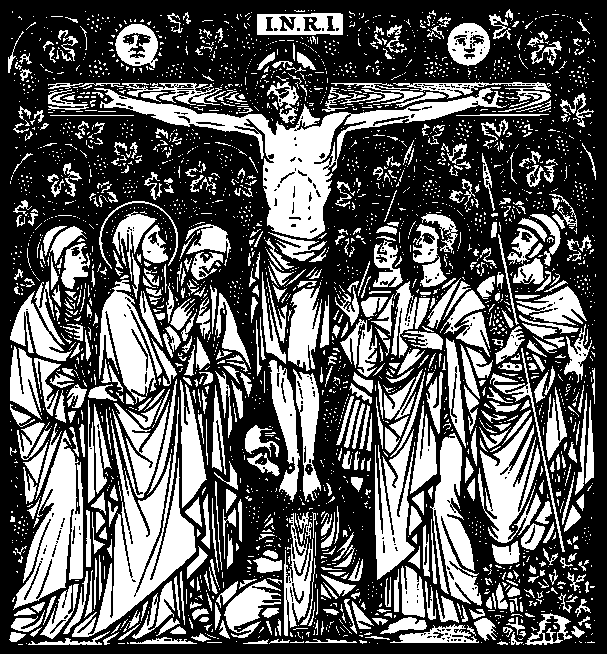
\includegraphics[width=0.44\textwidth]{../Images/Friday.pdf}
\end{center}
\vfill

%
% \newpage

\begin{center}
\phantom{Ad maiorem Dei gloriam}

\vspace{1.0cm}

{\Huge\scshape\textls[150]{\MakeLowercase{Appendix}}}\pdfbookmark[section]{Appendix}{appendix}

\vspace{1.0cm}
\end{center}

\bisubsection{Responsorium breve}{Short response}\label{ResponsoriumBreveAlt}

\bimusichangingdouble[Feria V in Passione Domini terminans cum \textcolor{black}{\dots ad mortem,} sed et Feria VI terminans cum \textcolor{black}{\dots autem crucis,} et, cum dicitur Sabbato Sancto, terminans cum \textcolor{black}{\dots omne nomen.}][On Maundy Thursday, ending with \textcolor{black}{\dots death,} and Good Friday, ending with \textcolor{black}{\dots on a cross,} and, when said on Holy Saturday, ending with \textcolor{black}{\dots all other names.}]{\gregorioscore{../Responsories/ChristusFactusEst_OCO_as_vespers-simpler-neumes.gabc}}{Christ humbled himself for us and, in obedience, accepted death, \GreStar\,even death on a cross. \GreStar\GreStar\,Therefore God raised him to the heights and gave him the name which is above all other names.}

\bimusichangingdouble[Vel, in tono alio:][Or, in another tone:]{\gregorioscore{../Responsories/ChristusFactusEst_OCO_vel_option.gabc}}{Christ humbled himself for us and, in obedience, accepted death, \GreStar\,even death on a cross. \GreStar\GreStar\,Therefore God raised him to the heights and gave him the name which is above all other names.}

\bisubsection{Canticum envangelicum \textemdash{} Christus lumen gentium et gloria Israel}{Gospel canticle \textemdash{} Christ is the light of the nations and the glory of Israel}

\biinstruction{Antiphonæ ad libitum ad canticum \textcolor{black}{Nunc dimittis} possunt sumi ex sequentibus:}{Antiphons can be taken as desired for the canticle \textcolor{black}{Nunc dimittis} from the following:}\label{NuncDimittisAlt}

\bimusic[In dominicis vel tempore paschali:][On Sundays or in Easter time]{\gregorioscore{../NuncDimittis/11216-an--vigilemus_omnes--verona,DomTPCN.gabc}}{\GreColored{Ant.} Let us all keep watch with Christ, and always go the Lord with fear; for he is the strong lion who rose, and he has conquered the ancient serpent, alleluia.}

\bimusichangingdouble{\gregorioscore{../NuncDimittis/Nunc-dimittis-3b.gabc}}{At last, \GreColored{\grecross}\, all-powerful Master,\\
you give leave to your servant\\
to go in peace, according to your promise.\\

For my eyes have seen your salvation\\
which you have prepared for all nations,\\
the light to enlighten the Gentiles\\
and give glory to Israel, your people.\\

Glory be to the Father and to the Son\\
and to the Holy Spirit.\\
As it was in the beginning,\\
is now, and ever shall be,\\
world without end. Amen.}

\bimusic{\gregorioscore{../NuncDimittis/11216-an--vigilemus_omnes--verona,DomTPCN.gabc}}{\GreColored{Ant.} Let us all keep watch with Christ, and always go the Lord with fear; for he is the strong lion who rose, and he has conquered the ancient serpent, alleluia.}

\bimusic[In feriis:][On weekdays:]{\gregorioscore{../NuncDimittis/11217-an--gregem_tuum--verona,ferTpACN.gabc}}{\GreColored{Ant.} Never desert your flock, O Lord, good Shepherd, who know not sleep, but always keep watch.}

\bimusichangingdouble{\gregorioscore{../NuncDimittis/Nunc-dimittis-3b.gabc}}{At last, \GreColored{\grecross}\, all-powerful Master,\\
you give leave to your servant\\
to go in peace, according to your promise.\\

For my eyes have seen your salvation\\
which you have prepared for all nations,\\
the light to enlighten the Gentiles\\
and give glory to Israel, your people.\\

Glory be to the Father and to the Son\\
and to the Holy Spirit.\\
As it was in the beginning,\\
is now, and ever shall be,\\
world without end. Amen.}

\bimusic{\gregorioscore{../NuncDimittis/11217-an--gregem_tuum--verona,ferTpACN.gabc}}{\GreColored{Ant.} Never desert your flock, O Lord, good Shepherd, who know not sleep, but always keep watch.}

\bimusic[In feriis:][On weekdays:]{\gregorioscore{../NuncDimittis/11218-an--lucem_tuam--verona,ferTpACN.gabc}}{\GreColored{Ant.} O Lord, grant us your light, that with the darkness of our hearts destroyed, we may be able to come to the light which is Christ.}

\bimusichangingdouble{\gregorioscore{../NuncDimittis/Nunc-dimittis-4e.gabc}}{At last, \GreColored{\grecross}\, all-powerful Master,\\
you give leave to your servant\\
to go in peace, according to your promise.\\

For my eyes have seen your salvation\\
which you have prepared for all nations,\\
the light to enlighten the Gentiles\\
and give glory to Israel, your people.\\

Glory be to the Father and to the Son\\
and to the Holy Spirit.\\
As it was in the beginning,\\
is now, and ever shall be,\\
world without end. Amen.}

\bimusic{\gregorioscore{../NuncDimittis/11218-an--lucem_tuam--verona,ferTpACN.gabc}}{\GreColored{Ant.} O Lord, grant us your light, that with the darkness of our hearts destroyed, we may be able to come to the light which is Christ.}

\bimusic[In feriis:][On weekdays:]{\gregorioscore{../NuncDimittis/11219-an--pacem_tuam--verona,ferTpACN.gabc}}{\GreColored{Ant.} We beseech your peace, O Lord, and may your peace, O Christ, remain in our spirits; that we may not fear the terror of the night, but may we always keep watch in all the works of your commandments.}

\bimusichangingdouble{\gregorioscore{../NuncDimittis/Nunc-dimittis-4e.gabc}}{At last, \GreColored{\grecross}\, all-powerful Master,\\
you give leave to your servant\\
to go in peace, according to your promise.\\

For my eyes have seen your salvation\\
which you have prepared for all nations,\\
the light to enlighten the Gentiles\\
and give glory to Israel, your people.\\

Glory be to the Father and to the Son\\
and to the Holy Spirit.\\
As it was in the beginning,\\
is now, and ever shall be,\\
world without end. Amen.}

\bimusic{\gregorioscore{../NuncDimittis/11219-an--pacem_tuam--verona,ferTpACN.gabc}}{\GreColored{Ant.} We beseech your peace, O Lord, and may your peace, O Christ, remain in our spirits; that we may not fear the terror of the night, but may we always keep watch in all the works of your commandments.}

\newpage

\bisubsection{Antiphona marialis}{Marian antiphon}

\subsubsection{Salve Regina}\label{SalveAlt}

\bimusichangingdouble[Post Dominicam Pentecostes:][After Pentecost Sunday:]{\verticalspacer\gregorioscore{../MarianAntiphons/2715-an--salve_regina--solesmes_1961-no-signs.gabc}}{Hail holy queen, mother of mercy\,: \\
Hail our life, our sweetness, and our hope.\\
To thee do we cry, poor banished children of Eve.\\
To thee do we send up our sighs, mourning and weeping in this vale of tears.\\
Turn then most gracious advocate, thine eyes of mercy towards us.\\
And after this, our exile, show unto us the blessed fruit of thy womb, Jesus.\\
O clement\,: O loving\,: O sweet Virgin Mary.}

\vfill
\begin{center}
  \includegraphics[width=0.44\textwidth]{../Images/MaryOther.pdf}
\end{center}
\vfill


\end{document}
